% https://mirror.hmc.edu/ctan/macros/latex/contrib/mnras/mnras_guide.pdf
% equation~(\ref{eq:quadratic}).
% Fig.~\ref{fig:example_figure}.
% Table~\ref{tab:example_table}.


% mnras_template.tex
%
% LaTeX template for creating an MNRAS paper
%
% v3.0 released 14 May 2015
% (version numbers match those of mnras.cls)
%
% Copyright (C) Royal Astronomical Society 2015
% Authors:
% Keith T. Smith (Royal Astronomical Society)

\documentclass[a4paper, fleqn, usenatbib]{mnras}

\usepackage[T1]{fontenc}
\usepackage{ae,aecompl}

\usepackage{graphicx} % Including figure files
\usepackage{amsmath}  % Advanced maths commands
\usepackage{amssymb}  % Extra maths symbols

\usepackage{booktabs}        % Table mid-rule line
\usepackage{mathtools}       % Curly braces above equation
\usepackage{pdflscape}       % Landscape tables
% \usepackage[hyphens]{url}    % Long URLs

\graphicspath{{./figs/}}

\defcitealias{ivison16}{Paper~I}
\defcitealias{lewis17}{Paper~II}

\newcommand{\hermes}{\textit{Her}MES}
\newcommand{\herschel}{\textit{Herschel}}

\newcommand{\angstrom}{\text{\AA}}
\newcommand{\kiloparsec}{\text{kpc}}
\newcommand{\megaparsec}{\text{Mpc}}

\newcommand{\fidelity}{\mathcal{F}}
\newcommand{\lfir}{L_{\text{FIR}}}
\newcommand{\lsol}{L_{\sun}}
\newcommand{\magab}{\text{mag}_{\text{AB}}}
\newcommand{\millijanksy}{\text{mJy}}
\newcommand{\mdust}{M_{\text{dust}}}
\newcommand{\mhalo}{M_{\text{halo}}}
\newcommand{\msol}{M_{\sun}}
\newcommand{\mstars}{M_{\text{stars}}}
\newcommand{\pur}{P_{\text{UR}}}
\newcommand{\reff}{R_{\text{eff}}}
\newcommand{\scuba}{\mbox{\textsc{Scuba}-2}}
\newcommand{\urg}{ultra-red galaxy}
\newcommand{\urgs}{ultra-red galaxies}
\newcommand{\znir}{z_{\text{NIR}}}
\newcommand{\zfir}{z_{\text{FIR}}}
\newcommand{\zphot}{z_{\text{phot}}}
\newcommand{\zspec}{z_{\text{spec}}}

\title[The Red Sequence is Emerging at a Faster Rate Around Ultra-Red Galaxies]{The Red Sequence is Emerging at a Faster Rate Around Ultra-Red Galaxies than in the Field}

\author[A.~J.~R.~Lewis et al.]{
% A.~J.~R.~Lewis,$^{1}$\thanks{E-mail: }
A.~J.~R.~Lewis,
R.~J.~Ivison,$^{1,2}$
P.~N.~Best,$^{1}$
M.~Bremmer,${?}
J.~E.~Geach,$^{?}$
I.~Oteo,$^{?}$
J.~M.~Simpson,$^{?}$
A.~Weiss$^{?}$\\
$^{1}$Institute for Astronomy, University of Edinburgh, Royal Observatory, Blackford Hill, Edinburgh EH9 3HJ, UK\\
$^{2}$European Southern Observatory, Karl Schwarzchild Stra{\ss}e 2, D-85748 Garching, Germany
}

\date{Accepted XXX. Received YYY; in original form ZZZ}

\pubyear{2018}

\begin{document}
\label{firstpage}
\pagerange{\pageref{firstpage}--\pageref{lastpage}}
\maketitle

\begin{abstract}
We selected a sample of $64$ ultra-red galaxies formation the S2CLS and S2COSMOS imaging surveys based on their \herschel{} photometry at their \scuba{} positions.
Uniformly deep and wide $850\text{-}\micron{}$ data around their environments suggests that just over half of these ultra-red galaxies reside in over-dense regions of DSFGs -- predominately residing near the centres ($<$ a few megaparsec) of over-densities.
Weighting each surrounding DSFG by its association probability to its central ultra-red galaxy, we found that the average total dust mass was $\sim2\times10^{9}\,\msol{}$ -- consistent with the values reported in the literature and the concept that they will evolve from high redshift ($z>3\text{--}4$) into present-day ETGs in the cores of rich galaxy clusters.
%
Using optical/NIR ground-based data (down to $5\text{-}\sigma_{K}$ depths of $\lesssim24\,\magab{}$) for $42$ ultra-red galaxies we were able to associate an average of $\approx28$ LBGs to within $\lesssim5'$ of a given \urg{}.
These associated LBGs showed a factor of $\approx5\times$ and $3\times$ increase in stellar mass and absolute ($M_{B}-M_{I}$) colour respectively as their distance to the ultra-red galaxies decreased over $\approx500\,\text{kpc}$ (or $\approx2'$) scales -- suggesting that the red sequence is beginning to emerge around ultra-red galaxies at $z\sim3$ at a faster rate compared to the field.
%
With an average total stellar mass contribution to the ultra-red galaxy environments from the LBGs of $4.7\times10^{11}\,\msol{}$, and assuming that the ultra-red galaxies convert all of their molecular gas into stars, these candidate, high-redshift proto-clusters have the potential to form systems with stellar masses of at least $\mstars{}\sim10^{12}\,\msol{}$ by $z\sim0$.
\end{abstract}

\begin{keywords}
galaxies: clusters: general -- galaxies: high-redshift -- galaxies: starburst -- infrared: galaxies -- submillimeter: galaxies
\end{keywords}

\section{Introduction}

The advent of sophisticated, multiplexed, bolometer arrays sensitive to sub-millimetre (sub-mm) emission \citep{kreysa98, holland99} facilitated the discovery of so-called `dusty star-forming galaxies' (DSFGs) over two decades ago \citep{smail97, barger98, hughes98, eales99}.
%
Obscured by vast quantities of dust (carbonaceous and amorphous silicate grains), which efficiently re-processes the ultra-violet (UV) starlight from these galaxies into far-infrared (far-IR) thermal radiation, a given DSFG is capable of producing a  $\mstars{}\gtrsim10^{11}\text{-}\msol{}$ galaxy after an intense, merger-induced burst of star formation lasting for $t_{\text{burst}}\sim100\,\text{Myr}$ \citep{lapi14, aversa15}.
%
Hence, these galaxies have transformed our understanding of cosmic star formation rates (SFRs, or $\psi$), which until their discovery had been based predominantly on detections of UV and optically selected `Lyman-break galaxies' \citep{steidel96, giavalisco02}.

Due to their rarity, however, generating large samples of DSFGs -- especially at the high-redshift ($z>4$) tail of this population -- requires expensive and time-consuming sub-mm imaging of large regions of the sky.
The arrival of the \herschel{} Space Observatory \citep{pilbratt10} alleviated this problem by allowing astronomers to simultaneously image large regions of the Universe at $250\text{-}$, $350\text{-}$ and $500\text{-}\micron{}$ wavelengths with its Spectral and Photometric Imaging Receiver \citep[SPIRE ---][]{griffin10} instrument.
These FIR observations provided a quick and relatively inexpensive means with which to generate a large sample of distant and/or colder DSFGs based on the location of the dust peak within their observed spectral energy distributions (SEDs\footnote{Since $\lambda_{\text{obs}}=(1+z)\lambda_{\text{rest}}\sim(1+z)\times100\,\micron{}$}).

In \citet[][hereafter \citetalias{ivison16}]{ivison16}, we followed-up a large sample of distant DSFGs -- or so-called `ultra-red galaxies' -- with \scuba{} \citep{holland13} from the largest ($\approx600\,\text{deg}^2$) imaging survey undertaken with \herschel{}, \textit{H}-ATLAS \citep[\herschel{}-Astrophysical Terahertz Large Area Survey ---][]{eales10}.
Our ultra-red galaxies were selected based on the following criteria:
\begin{align}
    \label{eq:ur_criteria}
    \overbrace{\left(S_{500}/S_{250}\ge1.5\right)\quad\land\quad\left(S_{500}/S_{350}\ge0.85\right)}^{\text{ultra-red}}\quad\land\hfill\\\nonumber
    \overbrace{\left(S_{500}\ge3.5\sigma_{500}\right)}^{\text{robust}}\quad\land\quad
    \overbrace{\left(S_{500}<100\,\text{mJy}\right)}^{\text{unlensed}},
\end{align}
\noindent
where `$\land$' is the logical `and' symbol.
Hence, equation~(\ref{eq:ur_criteria}) clearly selects very distant -- ergo ultra-red \citep{cox11} -- robust and largely unlensed \citep{negrello10} DSFGs.

In \citetalias{ivison16}, we showed that ultra-red galaxies have a median redshift of $z\approx3.7$ and a $z>4$ space density of $\rho\approx6\times 10^{-7}\,\text{Mpc}^{-3}$ -- the latter being consistent with their evolution into the most massive ($\mstars{}>10^{11}\,\msol$) NIR-selected galaxies at $z\sim3.5$ \citep{straatman14}.

Thus, being the likely progenitors to such massive galaxies suggests that ultra-red galaxies could play an important role in the evolution and formation of large structure, i.e.\ galaxy clusters, within the Universe.
The cores of such structures are rich with early-type galaxies (ETGs, i.e.\ relatively passive ellipticals and lenticulars) and mark the densest regions in the distribution of dark matter (DM).
These ETGs have commonly been viewed as transformed late-type galaxies (LTGs), which have had their star formation quenched via some environmental mechanism, leaving behind an ETG on the `red sequence' -- an empirical relation showing that brighter, ergo more massive, galaxies are typically redder with older stellar populations and less on-going star formation \citep{dressler97, bower98, baldry04, gerke07}.

Over-Dense regions are thought to have grown hierarchically since the decoupling of photons and matter, with initial peak positions supposedly etched into the Universe at some arbitrarily early epoch \citep{peebles70, spergel03}.
In the local Universe, galaxy clusters harbour the majority of ETGs, which in turn harbour over half of the present-day stellar mass.
Thus studying their cosmic evolution can place valuable constraints on models of galaxy formation \citep{springel05, robertson07, overzier09a}.

Therefore, in \citet[][hereafter \citetalias{lewis17}]{lewis17} we studied the $5\text{-arcmin}$, far-IR environments around a representative sub-sample of ultra-red galaxies at $z\gtrsim3$ to see if they are consistent with those expected for distant `proto-clusters' -- early over-densities that represent the precursors to modern-day galaxy clusters.

In \citetalias{lewis17} we showed that the FIR environments around \urgs{} are rich with bright ($S_{870}>8\,\millijanksy{}$) DSFGs compared to the field.
This suggested that ultra-red galaxies could signpost candidate proto-clusters at high redshift.

Thus, these results provide a relatively straight-forward approach to expanding the currently short list of known proto-clusters, i.e.\ by searching around the environments of ultra-red galaxies.

This motivates us in this paper to increase the number of potential proto-clusters by searching for ultra-red galaxies in the S2CLS and S2COSMOS imaging surveys.
The $850\text{-}\micron{}$ data for these two surveys are deeper and wider than those examined in \citetalias{lewis17}, which will allow us to improve upon the far-IR results reported previously.
Furthermore, complementary ground-based optical/near-IR catalogues will allow us to go one step further than in \citetalias{lewis17} and isolate any optical/near-IR galaxies around the \urgs{} that are associated to them.
We will examine whether these surrounding galaxies show traits consistent with residing in an over-dense environment at $z\gtrsim3\text{--}4$.
Such traits include being able to determine whether the formation of the red sequence is happening at a faster rate around \urgs{} than in the field, or whether there is any dependence on stellar mass with proximity to an \urg{}.
If optical/near-IR galaxies do not show such traits it may suggest that there is something incorrect with our understanding in the formation and evolution of massive galaxies as traced by distant DSFGs.

The structure of this paper is as follows.
In sections~2 and 3 we outline our ultra-red galaxy sample, as well as the far-IR analysis and results of this sample.
We present our optical/near-IR analysis, results and discussion in section~4, whilst summarising and presenting our conclusions in section~5.
Throughout our analysis and discussion, we adopt a `concordance cosmology' with $H_0=71\,\text{km}\,\text{s}{-1}\,\megaparsec{}^{-1}$, $\Omega_{m} = 0.27$ and $\Omega_\Lambda = 0.73$ \citep{hinshaw09}, in which $1'$ corresponds to a (proper) distance of $\approx0.5\,\megaparsec{}$ at $z = 3$.
For a quantity, $x$, we denote its mean and median values as $x$ and $x_{1/2}$, respectively.

% % In the following section, I will describe the \textsc{Scuba}-2 datasets used and the method that I adopted for selecting \urgs{}.
% % In \crefrange{sec:analysis_s2cls}{sec:analysis_optical_s2cls}, I will provide a detailed analysis of the optical-through-to-\fir{} environments around \urgs{}, concluding with a brief summary in \cref{sec:conclusion_s2cls}.

\section{FIR Analysis}
\label{sec:fir_analysis}

\subsection{FIR Data Acquisition and Manipulation}

We used the publicly available catalogues for the S2CLS\footnote{%
  \url{https://zenodo.org/record/57792\#.WOtnkRiZNE5}.}
\citep{geach17} and the \scuba{} Cosmic Evolution Survey (S2COSMOS --- Simpson et al., in prep.) imaging surveys to search for \urgs{}.

The former is comprised of seven extragalactic fields: the Akari-Northern Ecliptic Pole \citep[Akari-NEP ---][]{takagi09}, the Cosmological Evolution Survey \citep[COSMOS ---][which was further imaged during S2COSMOS]{scoville07}, the Extended Groth Strip \citep[EGS ---][]{groth94}, the Great Observatory Origins Deep Survey-North \citep[GOODS--N ---][]{wang04}, the Lockman Hole North \citep[LHN ---][]{dickey90}, the Small Selected Area 22 \citep[SSA~22 ---][]{lilly91} and the United Kingdom Infra-Red Telescope \citep[UKIRT ---][]{casali07} Infra-Red Deep Sky Survey-Ultra Deep Survey \citep[UKIDSS--UDS, or simply UDS ---][]{lawrence07}.
The FIR analysis that we performed required complementary \herschel{} data and we therefore discarded the Akari-NEP and SSA~22 fields as, to the best to our knowledge, the data for these fields are either too shallow or non-existent.
Thus, the five extragalactic fields analysed here cover a surveyed area of $\mathcal{A}\approx3.7\deg^2$ down to an instrumental r.m.s.\ of $\sigma_{\text{inst}}<1.6\,\millijanksy{}$.
This is a factor of $\sim4\times$ and $\sim2\times$ improvement on the area and sensitivity considered in \citetalias{lewis17}, respectively.
The S2CLS and S2COSMOS catalogues contain $1{,}207$ and $1{,}603$ sources above an $850\text{-}\micron$ SNR of $S/N>3.5$ and $S/N>4.0$, respectively.

\subsection{PACS and SPIRE Photometry}

FIR flux densities were measured on the \herschel{} PACS ($100$ and $160\,\micron{}$) and SPIRE ($250$, $350$ and $500\,\micron{}$) images with PSF FWHM of $\theta=7$ and $11.6\arcsec{}$ \citep{ibar10} and $18$, $24.8$ and $35.1\arcsec{}$ \citep{nguyen10}, respectively.
These images were accessed through the PACS Evolutionary Probe website\footnote{%
  \url{www.mpe.mpg.de/ir/Research/PEP/DR1}.}
\citep{lutz11} and the \herschel{} Database in Marseille, respectively.

We extracted $2\arcmin\times2\arcmin$ \herschel{} sub-images at the \scuba{} positions (which were catalogued in decreasing order of $850\text{-}\micron{}$ SNR) and subsequently performed a six-dimensional Gaussian fit using the \textsc{idl} \textsc{Mpfit} package \citep{markwardt09}.
During the fitting, we kept the \herschel{} FWHM fixed but allowed the Gaussian centroid ($\alpha,\delta$) to vary according to the $1\text{-}\sigma$ \scuba{} radial offset for a given \scuba{} source with a SNR given by:
\begin{equation}
    \label{eq:s2cls_radial_offset}
    \mathcal{R}_{\alpha} = \mathcal{R}_{\delta} = \frac{\mathcal{R}}{\sqrt{2}} \approx 11.2\arcsec{}(S/N)^{-1.6},
\end{equation}
\noindent
where $\mathcal{R}$ has been parameterised using \href{}{equation~(6)} in \citet{geach17} to yield a similar expression to that derived in \href{}{equation~(B22)} of \citet{ivison07}.
For each fit, we recorded the Gaussian peak flux density and corresponding $1\text{-}\sigma$ fitting error (both in units of $\millijanksy{}\,\text{beam}^{-1}$).
To these fitting errors, we added in quadrature the $\sigma$-clipped standard deviation of the extracted $2\arcmin{}\times2\arcmin{}$ sub-image for the PACS measurements and confusion noises\footnote{
  The SPIRE $250\text{-}$, $350\text{-}$ and $500\text{-}\micron{}$ confusion noises are $\sigma_{\text{conf}}=5.8$, $6.3$ and $6.8\,\millijanksy{}$, respectively \citep{nguyen10}.}
for the SPIRE measurements.

The resulting two-dimensional fits were then subtracted from their respective \herschel{} images -- effectively de-blending the \herschel{} images using a \scuba{} prior.
Finally, we made no attempt to fit multiple gaussians to the \herschel{} images in cases where the \scuba{} detections are within a \scuba{} PSF of each other.

\subsection{Ultra-Red Probability}

In \citetalias{lewis17}, we showed that not all of the central LABOCA sources were ultra-red after having their SPIRE photometry re-measured at their catalogued $870\text{-}\micron$ position.
This led to the introduction of a probability term that a DSFG is ultra-red ($\pur{}$), which we used to isolate a robust sub-sample of \urgs{}.
To recap, this `ultra-red probability' was derived by drawing $10{,}000$ Gaussian realisations of the SPIRE photometry for a given DSFG and determining the fraction of these realisations that satisfied equation~(\ref{eq:ur_criteria}).
This method allows us to generate a robust subset of \urgs{} that incorporates the photometric errors from \emph{all} SPIRE passbands.

\begin{figure}
    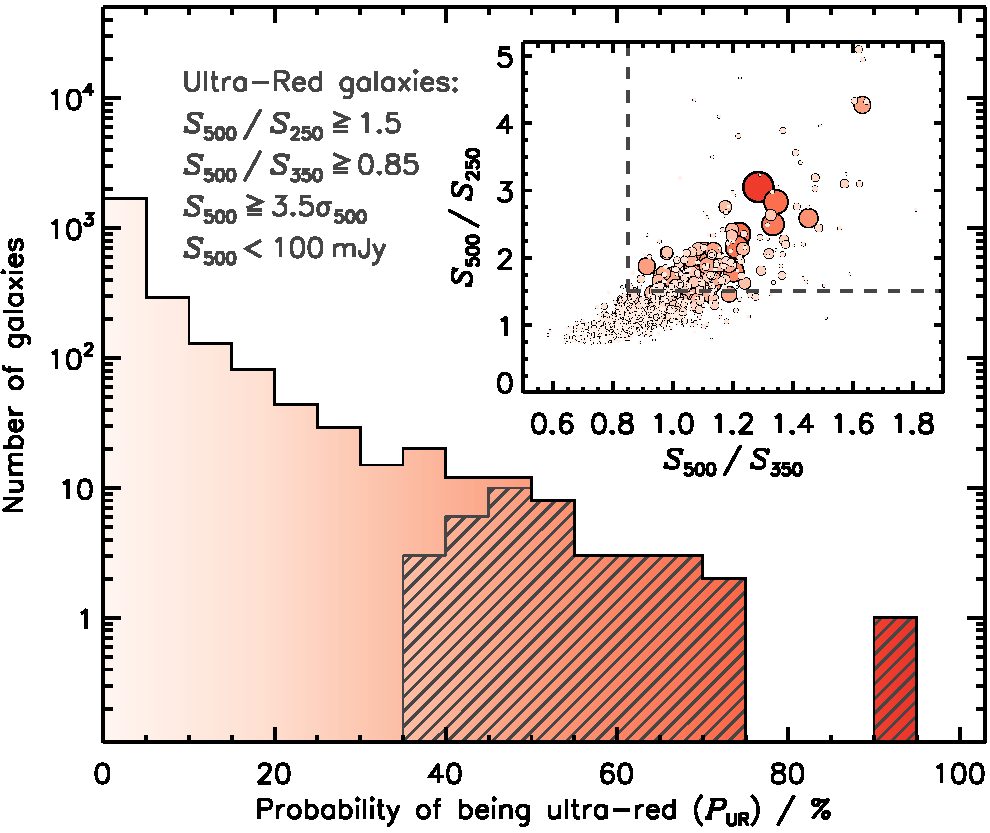
\includegraphics[width=\columnwidth]{prob_ur_s2}
    \caption{\textbf{Main:} histogram of the ultra-red probabilities for $\sim2{,}000$ DSFGs in the S2CLS and S2COSMOS imaging surveys.
    We colour-code this histogram from light-to-dark red as the ultra-red probability increases.
    The ultra-red criteria clearly selects the rarest DSFGs within these two surveys -- only a handful ($3$) have an ultra-red probability above $>68.27\%$.
    The dark-grey shaded histogram represents the $39$ DSFGs with SPIRE flux densities that directly satisfy equation~(\ref{eq:ur_criteria}).
    This motivated us to define an `\urg{}' as a galaxy that has an ultra-red probability above $>35\%$, which $64$ galaxies satisfy.
    \textbf{Inset:} $S_{500}/S_{350}$ versus $S_{500}/S_{250}$, colour-coded and scaled such that redder/larger circles have a higher ultra-red probability.
    The DSFG with the highest ultra-red probability, S2COSMOSJ100249$+$023255, has SPIRE flux-density ratios of $S_{500}/S_{250}\approx3$ and $S_{500}/S_{350}\approx1.3$ and a photometric redshift consistent with it being at $z\sim4$.
    \textbf{Note.\ } Black dashed lines represent the ultra-red colour-cut boundaries.
    }
    \label{fig:prob_ur_s2}
\end{figure}

In Fig.~\ref{fig:prob_ur_s2}, we show the ultra-red probability for $\sim2{,}000$ DSFGs in the S2CLS and S2COSMOS imaging surveys.
Motivated by the dark-grey shaded region in this figure, which represents those DSFGs whose mean SPIRE values suggest that they are ultra-red, we considered all galaxies with $\pur{}>35\%$ as being ultra-red.
At this probability threshold, Fig.~\ref{fig:prob_ur_s2} indicates that there is a significant fraction ($25$) of DSFGs that are not directly classified as being ultra-red based on their mean SPIRE flux densities.
These DSFGs are either just under the colour-cut limits and/or have larger SPIRE flux-density uncertainties.

In total, we provide a sample of $64$ \urgs{}, primarily from the COSMOS ($\approx60\%$) and UDS ($\approx30\%$) fields and the remaining from the EGS ($\approx5\%$), GOODS-N ($\approx2\%$) and LHN ($\approx2\%$) fields.
    %\footnote{%
    % In \citet{ivison16}, we analysed \urgs{} from a parent sample of $7{,}961$ detections, which was $77\%$ complete.
    % Given that the \textit{H}-ATLAS imaging survey covers a factor of $\approx160\times$ more area, we would expect to uncover $7{,}961/0.77/160\approx65$ \urgs{} within the area analysed here, which we do.}

\begin{table}
    \centering
    \caption{The number of DSFGs versus ultra-red probability threshold.}
    \label{tab:number_of_ur}
    \begin{tabular}{lccc}
        \hline
        Field & \multicolumn{3}{c}{\dotfill\,$N(>\pur{}\,/\,\%)$\,\dotfill} \\
        & $>0$ & $>35$ & $>68.27$\\
        \hline
        COSMOS & $1{,}043$ & $38$ & $2$\\
        EGS & $186$ & $3$ & $0$\\
        GOODS-N & $57$ & $1$ & $0$\\
        LHN & $189$ & $1$ & $0$\\
        UDS & $876$ & $21$ & $1$\\\cmidrule[0.5pt]{2-4}
        & $\boldsymbol{2{,}351}$ & $\boldsymbol{64}$ & $\boldsymbol{3}$\\
        \hline
    \end{tabular}
\end{table}

In Table~\ref{tab:number_of_ur}, we show how the number of \urgs{} varies as we change the ultra-red probability threshold.
Despite having set a fairly lenient threshold, the sample of \urgs{} with $\pur{}>35\%$ that we present only accounts for $\approx3\%$ of the total number of sources catalogued across both of the imaging surveys.
If we were to enforce a stricter, more robust threshold of $\pur{}\gtrsim68\%$, we would only be left with a sample of three \urgs{} -- reflecting the fact that \urgs{} become exponentially rarer with increasing ultra-red probability.
However, such a small sample of robust \urgs{} prohibits any meaningful statistical analysis, which justifies the adoption of a less conservative ultra-red probability threshold in this work.
Finally, it is worth mentioning that we only used the ultra-red probability to select a sample and not as a weighting for the properties analysed.

\subsection{FIR Photometric Redshifts}

We combined the PACS, SPIRE and \scuba{} flux-density measurements in order to determine FIR photometric redshifts for all $\sim2{,}000$ DSFGs.
We added in quadrature the confusion noise \citep[$\sigma_{\text{conf}}=0.8\,\millijanksy$ ---][]{geach17} \emph{and} calibration error ($\sigma_{\text{cal}}=0.048S_{\text{inst}}$, where $S_{\text{inst}}$ is the instrumental flux density) to the de-boosted instrumental $850\text{-}\micron{}$ uncertainties.
The calibration uncertainty -- derived from the $1\text{-}\sigma$ scatter in the peak flux conversion factors of $>500$ calibrator sources \citep{dempsey13} -- increases the unrealistically small measurement errors for bright (likely lensed) DSFGs.

FIR photometric redshifts were derived in a similar fashion to that described in \citetalias{ivison16} and \citetalias{lewis17}.
To recap, we used three template SEDs (ALESS, the Cosmic Eyelash, and \citet{pope08}) and adopted the template that produces the lowest $\chi^2$ over a redshift interval of $0<\zphot{}<10$ (down to a resolution of $\delta \zphot{} =0.01$).
In all further analysis, we used the resulting photometric redshift distribution ($P(z)$) for this best template\footnote{%
    These distributions were `dilated' to take into account the template-to-template scatter in the best-fitting redshift estimates for each DSFG.
}, which was derived from the best-fitting redshift values to $1{,}000$ realisations of the FIR photometry.
Adopting the entire photometric redshift distribution accounts for the (sometimes) complex shapes that they may possess better than simply adopting a Gaussian representation for them.

Finally, we draw attention to $459$ DSFGs ($\approx16\%$ of the sample) that were excluded from further analysis as their best-fitting photometric redshift values are within $\pm1\sigma$ of a grid boundary, i.e.\ $\sigma^{-}<\zphot{}<10-\sigma^{+}$.
These sources have a median $850\text{-}\micron{}$ SNR and stacked de-boosted flux density of $S/N\approx4$ and $S_{850}=3.4\pm0.1$, respectively.
However, they are undetected in both PACS and SPIRE, with stacked flux densities of $S_{100}=0.0\pm0.1\,\millijanksy{}$, $S_{160}=-0.5\pm0.3\,\millijanksy{}$, $S_{250}=-0.5\pm0.2\,\millijanksy{}$, $S_{350}=-0.5\pm0.2\,\millijanksy{}$ and $S_{500}=-0.7\pm0.2\,\millijanksy{}$. 
Therefore, it seems plausible that these \herschel{} undetected sources are perhaps spurious (or very faint), which justifies the decision not to include them in any further analysis.
The final sample is now based on a reduced sub-sample of $2{,}810-459=2{,}351$ DSFGs across the two imaging surveys.

\begin{figure}
    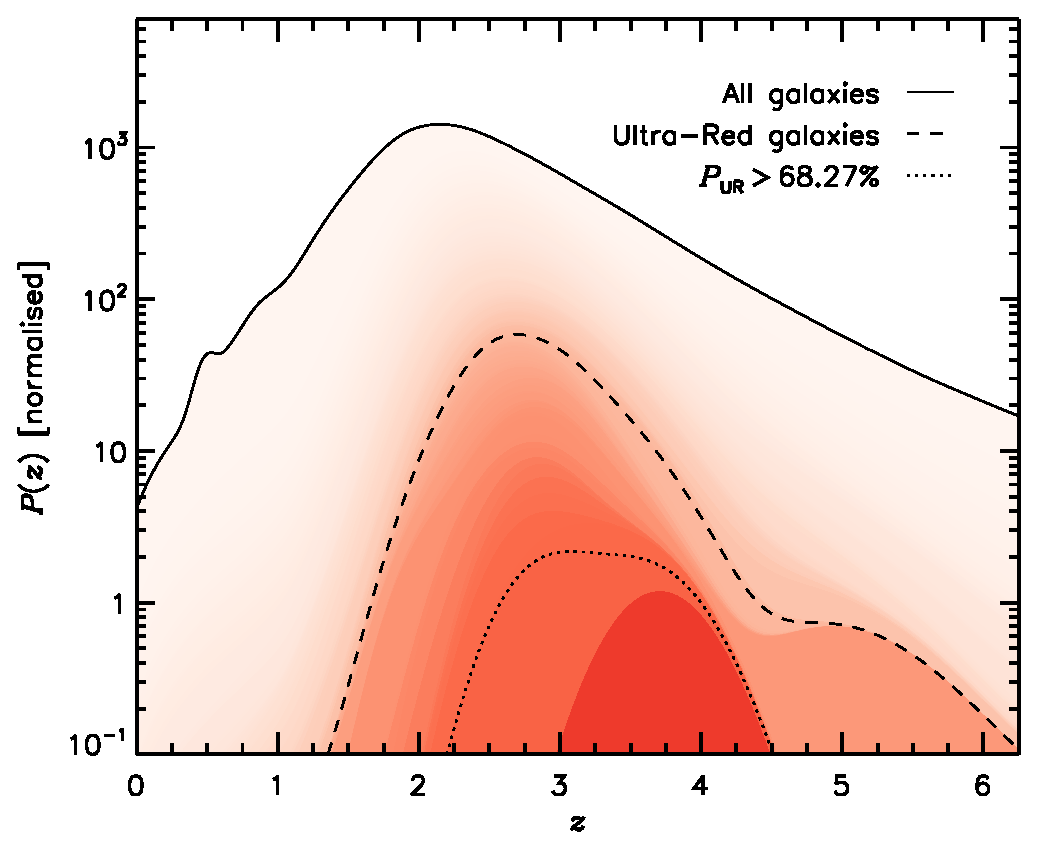
\includegraphics[width=\columnwidth]{photoz_s2}
    \caption{Sum of the photometric redshift distributions for all DSFGs (black solid line), ultra-red ($>35\%$, black dashed line) and the robust ultra-red ($>68.27\%$, black dotted line) galaxies.
    We have coloured-coded this figure such that redder colours represent the sum of the photometric redshift distributions for galaxies above a given ultra-red probability, as in Fig.~\ref{fig:prob_ur_s2}.
    The general population is peaked at $z\sim2$, whilst the \urg{} sample is shifted to $z\sim3$.
    Not every DSFG above $z\gtrsim3$ is contained within the \urg{} sample, as many of these are likely lensed \citep[$S_{500}\ge100\,\millijanksy{}$, e.g.][]{ikarashi11} or have poorly constrained SPIRE photometry.
    Although a very small sub-sample, the robust \urgs{} are peaked closer to $z\approx3.5$ -- in strong agreement with the rigorously `eyeballed' \urgs{} in \citetalias{ivison16}.
    The reddest photometric redshift belongs to the most robust \urg{} in the sample presented here, S2COSMOSJ100249$+$023255.}
    \label{fig:photoz_s2}
\end{figure}

In Fig.~\ref{fig:photoz_s2}, we show how the sum of the photometric redshift distributions varies as the ultra-red probability is changed -- highlighting where the ultra-red sub-sample and the three robust \urgs{} lie.
The general $850\text{-}\micron{}$-selected population peaks at $z\sim2$, whilst the \urg{} sample presented here is shifted to $z\sim3$ -- reinforcing the effectiveness of this colour-selection technique.
Interestingly, the more robust ($\pur{}>68.27\%$) \urgs{} peak even further at $z\approx3.5$ -- in good agreement with the results presented in \citetalias{ivison16}.
This reflects the smaller fraction of galaxies with (relatively) low ultra-red probabilities contained within the rigorously `eyeballed', \textit{H}-ATLAS sub-sample in \citetalias{ivison16} than compared to here.
Furthermore, this eyeballing stage, in conjunction with shallow $\sim850\text{-}\micron{}$ imaging, seems to have provided a higher fraction ($\approx40\%$) of robust ($\pur{}>68.27\%$) \urgs{} than presented here ($\approx5\%$).

Finally, we derived a FIR luminosity ($\lfir{}$) for each DSFG by integrating the best-fitting template SED across $8\text{--}1{,}000\,\micron{}$ in the rest frame.
We converted these FIR luminosities into SFRs using 
\begin{equation}
    \label{eq:sfr}
    \frac{\psi}{\msol{}\,\text{yr}^{-1}}\approx1.7\times10^{10}\frac{\lfir{}}{\lsol{}},
\end{equation}
which assumes a Salpeter initial mass function (IMF) for star-bursting galaxies \citep{kennicutt98}.

SFRs computed in this way are very sensitive to the underlying assumption made about the IMF.
For instance, if a Chabrier IMF \citep{chabrier03} is assumed, which exponentially decreases the number of low mass ($\le1\,\msol{}$) stars produced, then the results obtained by equation~(\ref{eq:sfr}) would be need to be scaled down by a factor of $\approx0.6\times$.
Furthermore, there is also growing support that the IMF may actually be `top heavy' within these dusty galaxies, i.e.\ for every high-mass star formed there would be many fewer low-mass stars formed \citep[][but see \citeauthor{hayward13}, \citeyear{hayward13}; \citeauthor{safarzadeh17}, \citeyear{safarzadeh17}]{baugh05, romano17, zhang18}.
This excess of high-mass stars also boosts the production of dust, which is necessary for increasing the FIR luminosity of these dusty galaxies.
If the IMF were top heavy, then the SFRs calculated with equation~(\ref{eq:sfr}) would be over-estimated by a factor of $\approx3\times$.

We also computed dust masses by re-arranging the standard expression for the flux density in the optically thin (to sub-mm emission) regime (i.e.\ the optical depth $\tau_{\nu}\ll1$):
\begin{equation}
    \label{eq:flux_density}
    S_{\nu}(1+z) = \left(1-e^{-\tau_{\nu}}\right)B_{\nu}(T)\Omega_s = \tau_{\nu}B_{\nu}(T)\Omega_s,
\end{equation}
where $B_{\nu}$ is the Planck function at a temperature $T$ and $\Omega_s=A/D_L^2$ is the solid angle of a DSFG with a projected area $A$ at a luminosity distance $D_L$.
Since the optical depth is related to the opacity ($\kappa_{\nu}$) and the surface area of dust mass ($\Sigma_{\text{dust}}$) as $\tau_{\nu}=\kappa_{\nu}\Sigma_{\text{dust}}$, equation~(\ref{eq:flux_density}) can be re-arranged to:
\begin{equation}
    \label{eq:dust_mass}
    \mdust{} = \Sigma_{\text{dust}}A = \frac{ S_{\nu} D_L^2 }{(1+z)\kappa_{\nu}B_{\nu}},
\end{equation}
where the factor of $(1+z)$ accounts for the band-shifting and compression of frequency space with redshift.
We used equation~(\ref{eq:dust_mass}) to determine the dust masses for all DSFGs with a photometric redshift.

\section{FIR Results, Analysis and Discussion}
\label{sec:fir_results}

We now provide an analysis on the FIR environmental properties around these $64$ \urgs{} within the S2CLS and S2COSMOS imaging surveys.
It is worth briefly mentioning that by analysing the environments around all \urgs{}, the results presented here should be free from publication bias.

\subsection{Galaxy-Centric Over-Density}

The first property that we considered was the galaxy-centric aperture over-density in order to examine the effectiveness of using \urgs{} to signposts distant, candidate proto-clusters down to a uniform flux-density limit.

To help decide on the size of the aperture with which to measure these over-densities, we turned to the work of \citet{chiang13}.
These authors analysed the redshift-dependent properties of $\sim3{,}000$ proto-clusters within the Millennium Simulation \citep{springel05}, which they divided into three resulting $z=0$ halo mass ($\mhalo^{z=0}$) bins representing Fornax- ($\mhalo^{z=0}=(1.37\text{--}3)\times10^{14}\,\msol{}$), Virgo- ($\mhalo^{z=0}=(3\text{--}10)\times10^{14}\,\msol{}$) and Coma-type ($\mhalo^{z=0}>10^{15}\,\msol{}$) galaxy clusters.
To quantify the spatial distribution that the smaller member halos occupied along the merger trees for a given proto-cluster at any given redshift, \citeauthor{chiang13} introduced an effective radius ($\reff{}$) defined as:
\begin{equation}
    \label{eq:effective_radius}
    \reff{}(z)=\sqrt{\frac{1}{\mhalo{}(z)}\sum_i\Delta r_{i}},
\end{equation}
\noindent
where $\mhalo{}(z)$ is the total halo mass at redshift $z$, the sum is over all smaller member halos and $\Delta r_{i}$ is the distance of each smaller member halo to the centre of mass of its respective proto-clusters.

Over the typical redshift range that \urgs{} subtend ($2\lesssim z \lesssim4$), the effective radius for the most massive present-day galaxy clusters varies from $4.9\arcmin{}\lesssim\reff{}\lesssim3.8\arcmin{}$.

Thus, in order to be sensitive to all proto-clusters with eventual halo masses that range from $\mhalo^{z=0}\approx10^{14}\text{--}10^{15}\,\msol{}$, we chose an aperture with size of $\reff{}=4.9\arcmin{}$, which we represented as a peak-normalised, two-dimensional Gaussian with a FWHM of $\theta=2\reff{}\approx10\arcmin{}$ ($\mathcal{G}_{\reff{}}$).

The number of surrounding galaxies around each catalogued DSFG ($\mathcal{N}_{\reff{}}$) was computed through a convolution between the aperture (centred on the position of a source) and a two-dimensional representation of these surrounding galaxies ($N$).
In this idealised representation, each surrounding galaxies was simulated as a two-dimensional Gaussian with a centroid equal to its catalogued position and a FWHM of $$\theta=\sqrt{8\ln(2)}\mathcal{R},$$ i.e.\ each DSFG was slightly `smeared' around its probable position, with the amount of smearing inversely proportional to its SNR (see equation~(\ref{eq:s2cls_radial_offset})).
These Gaussian representations were then normalised to their respective fidelity parameters using the catalogued FDR.
As in \citetalias{lewis17}, the signpost galaxy was removed during the measurement of $\mathcal{N}_{\reff{}}$ in order to mitigate the bias associated with imaging a region where a galaxy is known to reside.
 % (see Fig.~\ref{fig:}).

In order to measure the `expected' number of sources around each DSFG ($\mathcal{N}'_{\reff{}}$), we first generated a two-dimensional image for each field representing the expected number of sources at any given position.
This was achieved as follows:

\begin{enumerate}
    \item Using the best-fitting Schechter parameters to the differential number counts suitable for a given field, we derive the number of sources expected per unit area \emph{at} at a given flux density $N(S)$, allowing the flux-density to range from $S=0.2\text{--}20.0\,\millijanksy{}$.
    \item Then, at a given value $\sigma$ in the instrumental noise image of a given field, we measure how the completeness ($\mathcal{C}(S/\sigma)$) varies over this flux-density range.
    As this completeness was derived from simulations that used the SNR detection thresholds, it naturally accounts for the number of sources expected with low flux-density values.
    \item The sum across all flux densities of the completeness multiplied by the number counts yields the expected number of sources per unit area, at a given value $\sigma$.
    Extending this to all values in the instrumental noise image, and multiplying by the area that each value subtends (i.e.\ the area of a pixel, $\mathcal{A}_{\text{pix}}$), yields a two-dimensional representation of the number of sources expected at all positions within a given field, given by $$
        N'_{\text{field}}=\sum_\sigma\sum_S \mathcal{C}(S/\sigma)\mathcal{A}_{\text{pix}}N(S).$$
\end{enumerate}

The number of sources expected around each DSFG ($\mathcal{N}'_{\reff{}}$) is then simply the convolution of the aperture (centred on the position of that DSFG) with the applicable $N'_{\text{field}}$, or $$\mathcal{N}'_{\reff{}}=G_{\reff{}}*N'_{\text{field}}.$$

Finally, we scaled $\mathcal{N}'_{\text{field}}$ by $\sim84\%$ in order to account for the slight deficit caused by removing $\approx16\%$ of the sample with poorly constrained photometric redshifts.
To re-iterate, generating the expected numbers of sources in this way accounts for the varying instrumental noise across a given image and thus appropriately weights regions with high-/low-instrumental noise.

\begin{figure}
    \centering
    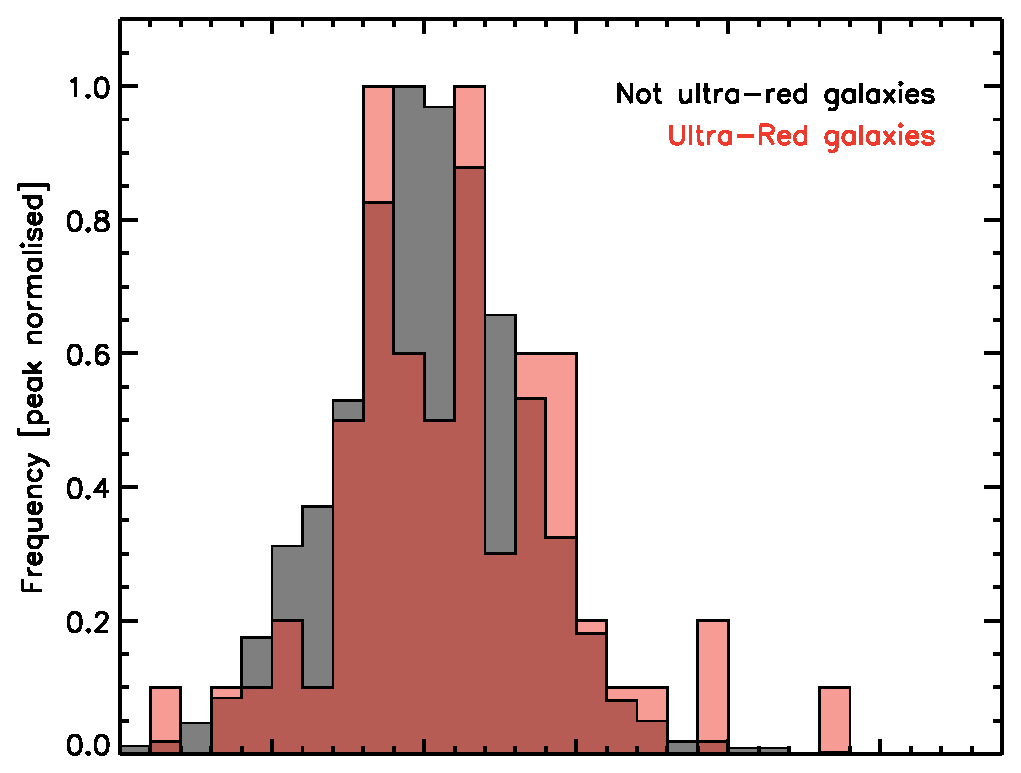
\includegraphics[width=\columnwidth]{overdensity_histogram}\\ %\vspace{1em}
    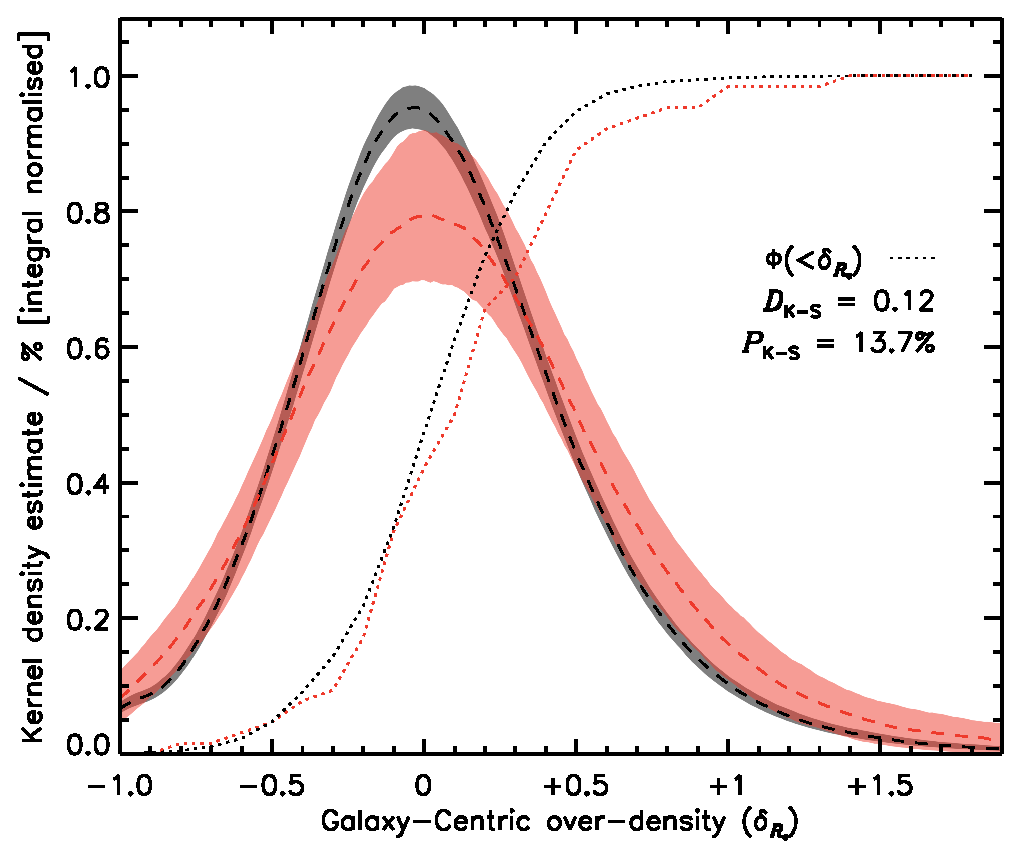
\includegraphics[width=\columnwidth]{overdensity_kernel_density_estimate}
    \caption{\textbf{Top:} peak-normalised histograms of the over-density parameter for ultra-red (red) and not ultra-red (black) galaxies.
    Each over-density parameter is calculated within an effective radius of $\reff{}\approx5\arcmin{}$ centred on each galaxy.
    We ensured that the central galaxy is removed from this calculation in order to reduce the galaxy-centric bias.
    The distribution for ultra-red galaxies appears to be slightly shifted towards higher over-density parameter values.
    \textbf{Bottom:} KDE of the over-density parameter for both samples derived by averaging $1{,}000$ realisations of the over-density parameter for each DSFG.
    The shaded regions represent the r.m.s.\ scatter across these realisations.
    A slight ($\gtrsim1\sigma$) excess is present in regions with higher ($\delta_{\reff{}}\gtrsim1$) over-density parameter values.
    Clearly not all ultra-red galaxies signpost over-dense regions, but there exists a growing separation between the two samples that becomes more pronounced around $\delta_{\reff{}}\approx0.5\text{--}1.5$.
    This indicates that \urgs{} preferentially signpost regions with greater over-density parameter values than galaxies that are not ultra-red, as found in the \citetalias{lewis17}.
    We over-plot the normalised CDFs (dashed lines) for these two samples, which highlights this divergence more clearly.
    A K-S test using the CDFs indicates that there is a $\approx15\%$ chance that the two distributions are the same.}
    \label{fig:over_density_parameter}
\end{figure}

In a similar method to \citetalias{lewis17}, we computed the galaxy-centric over-density parameter for each DSFG using:
\begin{equation}
    \label{eq:over_density_s2cls}
    \delta_{\reff{}}\equiv
    \frac{ (G_{\reff{}}*N) - (G_{\reff{}}*N'_{\text{field}})}
    {(G_{\reff{}}*N'_{\text{field}})}=\frac{\mathcal{N}_{\reff{}}}{\mathcal{N}'_{\reff{}}} - 1,
\end{equation}
where $G_{\reff{}}$ is the peak-normalised Gaussian aperture with a FWHM of $\theta=2\reff{}$, $N$ is the measured spatial distribution of all DSFGs excluding the central one, and $N'_{\text{field}}$ is the expected spatial distribution of galaxies, accounting for the varying instrumental noise values across a given field.

In Fig.~\ref{fig:over_density_parameter}, we show a histogram and kernel density estimate (KDE) of the over-density parameter for ultra-red and not ultra-red galaxy samples.
The KDE was computed by averaging many realisations of the over-density parameter for each DSFG and thus takes into account the uncertainties associated with each measurement.

We also show the normalised cumulative distribution functions (CDFs, or $\Phi$) for the the ultra-red ($\Phi_{\text{UR}}$) and not ultra-red ($\Phi_{\text{NUR}}$) galaxy samples, which we used to perform a two-sample Kolmogorov-Smirnov (K-S) test, defined as:
\begin{equation}
    \label{eq:ks_test}
    D_{\text{K-S}}=\sup_{\delta_{\reff{}}}|\Phi_{\text{UR}}\left(\delta_{\reff{}}\right)-\Phi_{\text{NUR}}\left(\delta_{\reff{}}\right)|,
\end{equation}
where $D_{\text{K-S}}$ is the maximum distance between the two CDFs.
This distance quantifies the probability that two CDFs are randomly drawn from the same population.

We derived a value of $D_{\text{K-S}}=0.12$, which equates to a probability of $P_{\text{K-S}}\sim15\%$ that ultra-red and not ultra-red galaxies are drawn from the same over-density parameter distribution.
Therefore, the differences are slight ($\gtrsim1\sigma$) between the two samples.
It appears that not all \urgs{} signpost over-dense regions and $\approx40\%$ of them lie in under-dense regions ($\delta_{\reff{}}\le0$) compared to $\approx50\%$ of the galaxies that are not ultra-red.
These results are somewhat similar to those found in \citetalias{lewis17} for bright ($S>8\,\millijanksy{}$) DSFGs.
% This result is similar to that found in the previous chapter for despite the (fairly) homogeneous instrumental noise images considered here.

\begin{figure*}
    \centering
    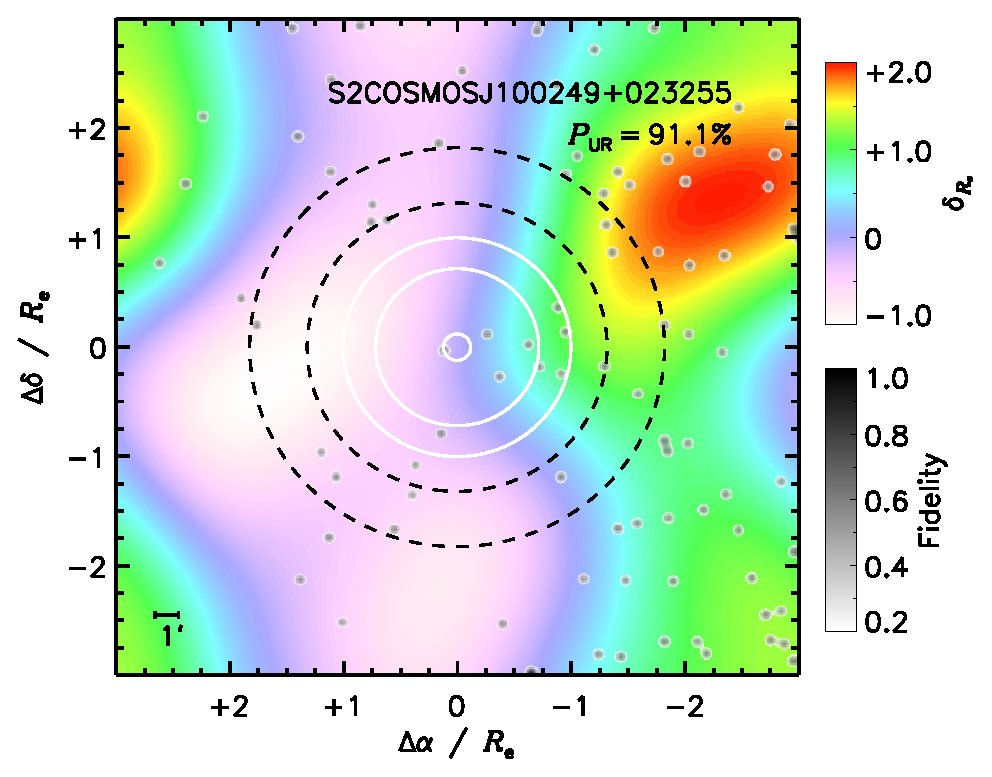
\includegraphics[width=0.5\textwidth]{S2COSMOSJ100249+023255-overdensity}
    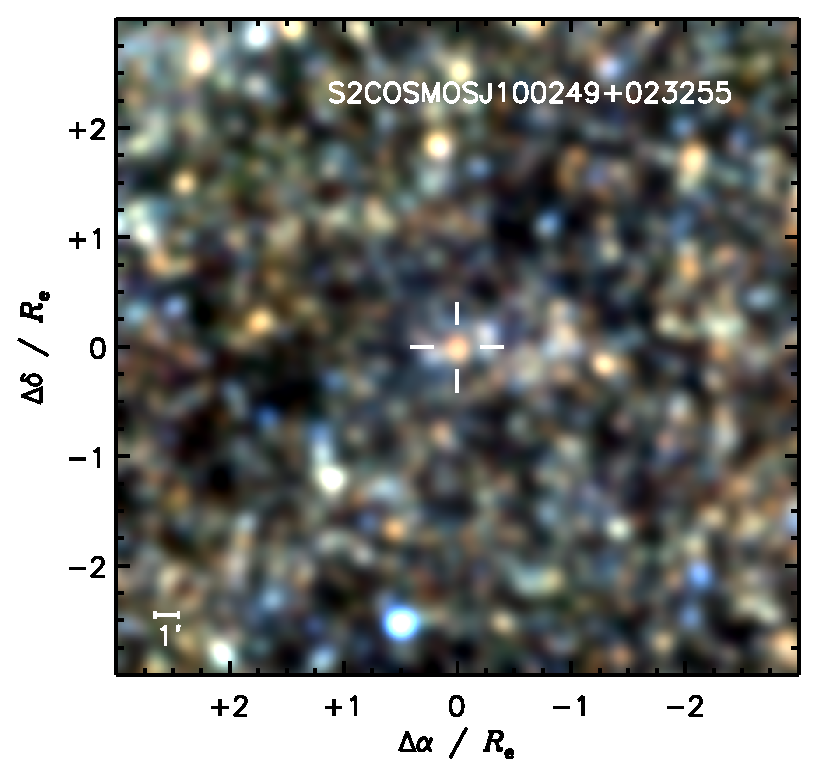
\includegraphics[width=0.41\textwidth]{S2COSMOSJ100249+023255-spire-rgb}\\\vspace{1em}
    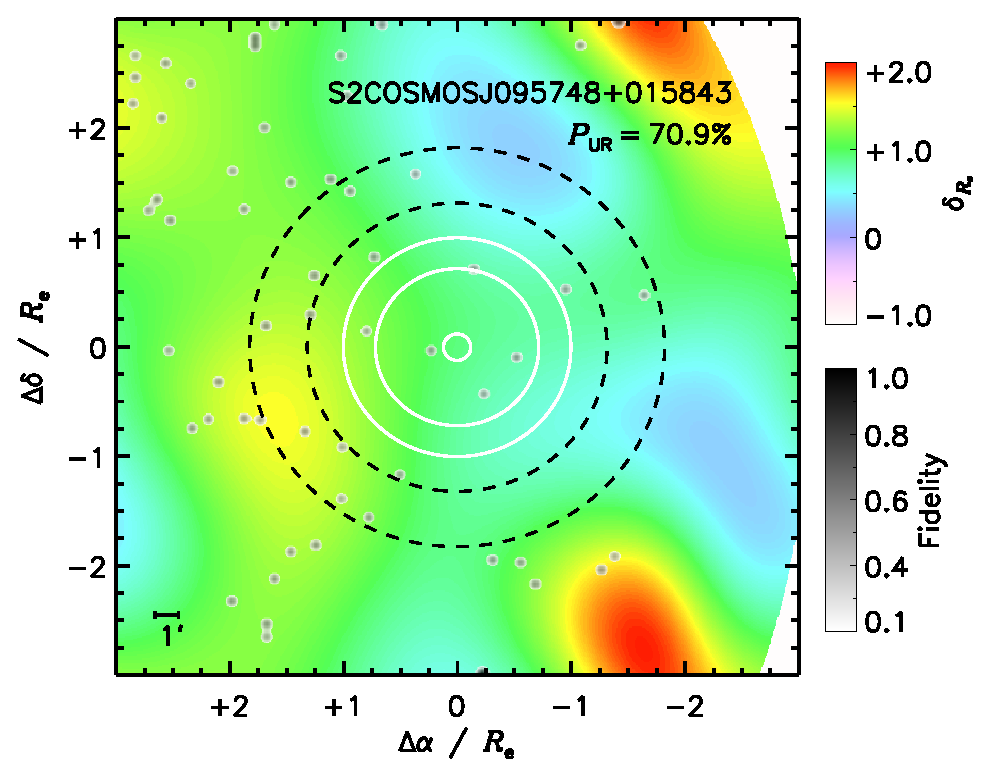
\includegraphics[width=0.5\textwidth]{S2COSMOSJ095748+015843-overdensity}
    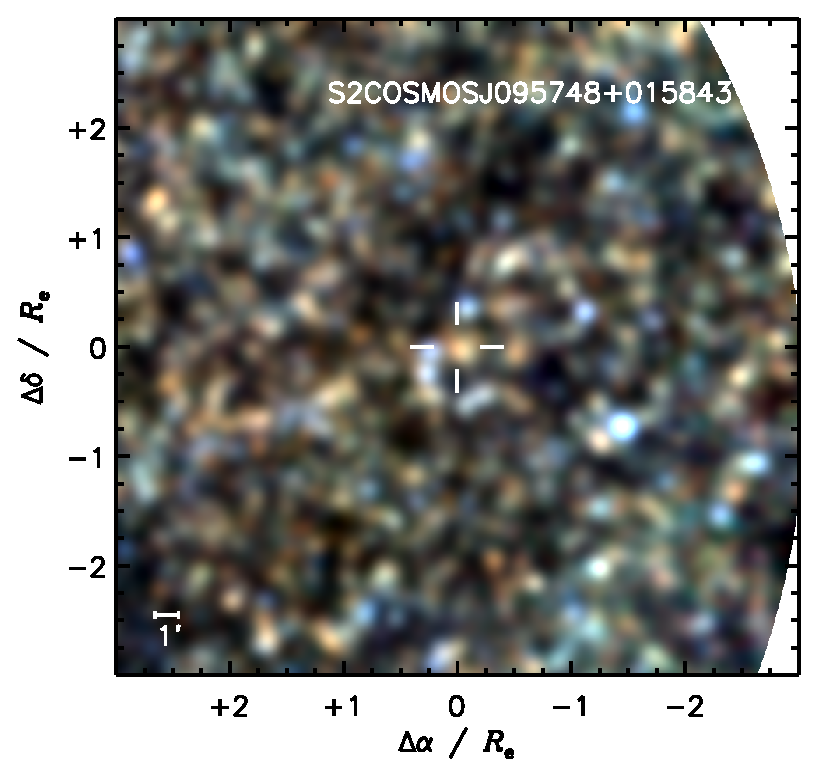
\includegraphics[width=0.41\textwidth]{S2COSMOSJ095748+015843-spire-rgb}\\\vspace{1em}
    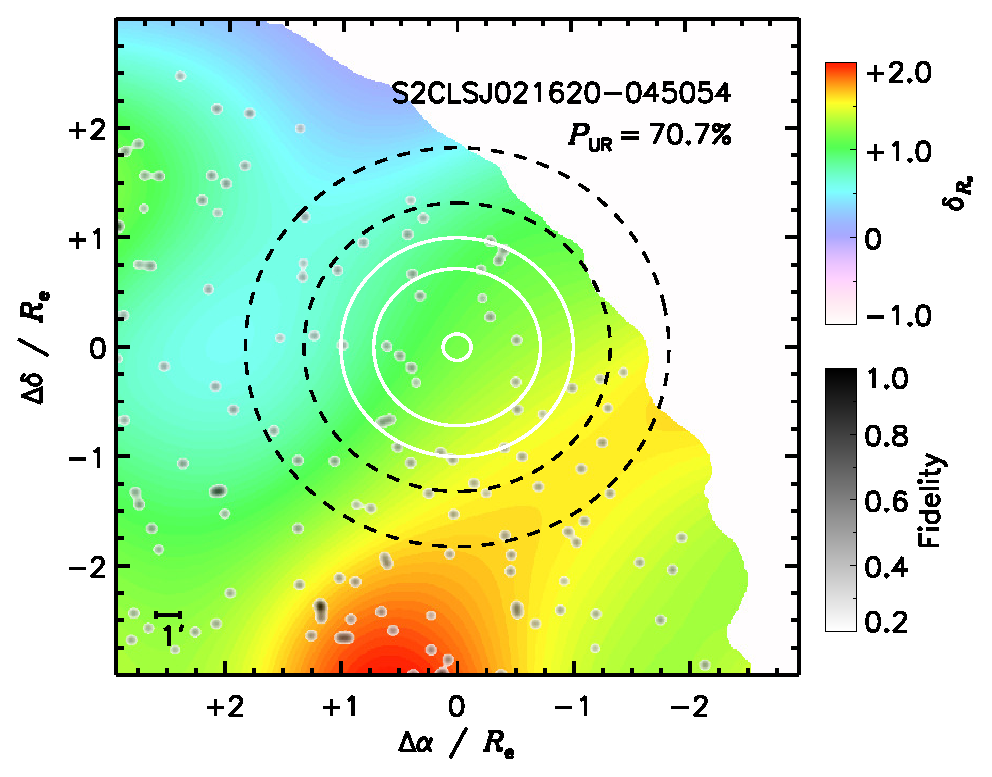
\includegraphics[width=0.5\textwidth]{S2CLSJ021620-045054-overdensity}
    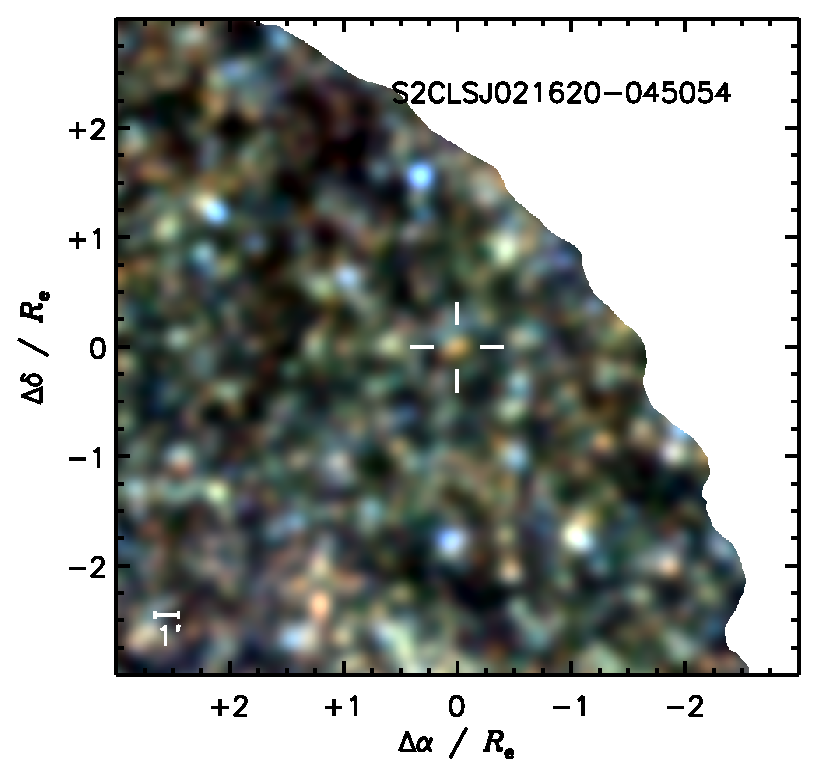
\includegraphics[width=0.41\textwidth]{S2CLSJ021620-045054-spire-rgb}
    \caption{\textbf{Left}: $6\reff{}\times6\reff{}$ cut-outs ($\reff{}\approx5\arcmin{}$) of the over-density parameter for galaxies with an ultra-red probability above $\pur{}>60\%$.
    These cut-outs are colour-coded such that bluer/redder regions represent lower/higher over-density values.
    Surrounding DSFGs are shown in black as Gaussian PSFs with FWHM of $\theta=14\arcsec{}$ that are integral normalised to their respective fidelity parameters.
    I show contours representing the $10$, $30$ (dashed black), $50$, $70$ and $99\%$ (white) values of the Gaussian aperture adopted, i.e.\ the aperture FHWM of $\theta=2\reff{}$ is indicated by the furthermost white contour.
    \textbf{Right}: SPIRE false-colour cut-outs of the same regions.
    The $250\text{-}$ and $350\text{-}\micron{}$ images have been filtered to the $500\text{-}\micron$ resolution.
    A white cursor indicates the central ultra-red galaxy within each cut-out.
    \textbf{Note}. --- Ultra-Red galaxies are presented in order of decreasing ultra-red probability.
    A distance scale is shown in the bottom left corner of each cut-out.
    This figure is continued in appendix~\ref{app:cut_outs} for the six extra \urgs{} with $\pur{}>60\%$.}
    \label{fig:s2cls_cut_outs}
\end{figure*}

Finally, Fig.~\ref{fig:s2cls_cut_outs}, which is continued in the appendix, shows the over-density and SPIRE false-colour cut-outs for \urgs{} with $\pur{}>60\%$.
The former indicate where the \urgs{} lie in relation to their closest over-density peaks.

\subsection{Proximity to Closest Over-Density Peak}

As discussed, $\approx60\%$ of \urgs{} reside in over-dense regions, which motivated us to examine the exact locations in these environments that they occupy.
For example, are these `over-dense' \urgs{} situated near to the centres of `high-value' over-density peaks, which would be consistent with them signposting the most extreme nodes in the DM distribution?
Or, is the situation closer to them signposting less extreme over-densities forming within the filamentary structure?

To answer this question, we used \emph{all} of the catalogued DSFGs in a given field to generate a `global' over-density image, which I used to search for `global peaks' that are above $\delta_{\reff{}}>0$.
These global peaks were detected and extracted using the same source extraction algorithm described in the \citetalias{lewis17}, i.e.\ searching for peaks in a top-down fashion that are separated by a distance of $2\reff{}$ from each other and the image edges.
The resulting global peaks were then normalised to the maximum value of the extracted peaks.
All extracted peaks were subsequently categorised as having either a low, medium or high value, corresponding to $0<\delta_{\reff{}}/\max{(\delta_{\reff{}})}<1/3$, $1/3<\delta_{\reff{}}/\max{(\delta_{\reff{}})}<2/3$ and $2/3<\delta_{\reff{}}/\max{(\delta_{\reff{}})}<1$, respectively.
We then analysed the radial distribution of \urgs{} to their closest global peak, under the assumption that medium-to-high-value global over-density peaks may represent extreme nodes in the DM distribution, whilst low-value global over-density peaks represent the less extreme over-densities with the filamentary structure.

In Fig.~\ref{fig:proximity}, we show this radial distribution for $\approx60\%$ of the \urgs{} that show a positive ($\delta_{\reff{}}>0$) over-density.
The closest global peaks to around $\sim2/3$ of these galaxies are of medium or high value.
All \urgs{} closest to a medium-value peak are distributed over $1.5\reff{}\approx7\arcmin{}$ (or $\sim3\,\megaparsec{}$ at $z=3$) scales, suggesting that they play a central role in these over-densities.
The situation is different for the high-value peaks as only $\approx65\%$ of the \urgs{} are distributed within $1.5\reff{}$ scales -- with some being as far out as $4\reff{}\approx15\arcmin{}$.

In the low-value peaks, which $\sim1/3$ of the $\approx60\%$ of \urgs{} occupy, they primarily tend to be within $0.5\reff{}$ (or $\sim1\,\megaparsec{}$ at $z=3$) of the peak position.
Thus, \urgs{} are mainly situated in the centres of low-valued over-density regions.
These findings may suggest that around $\approx20\%$ of \urgs{} are signposting less extreme over-densities within filamentary structures, rather than the extreme nodes.

\begin{figure*}
    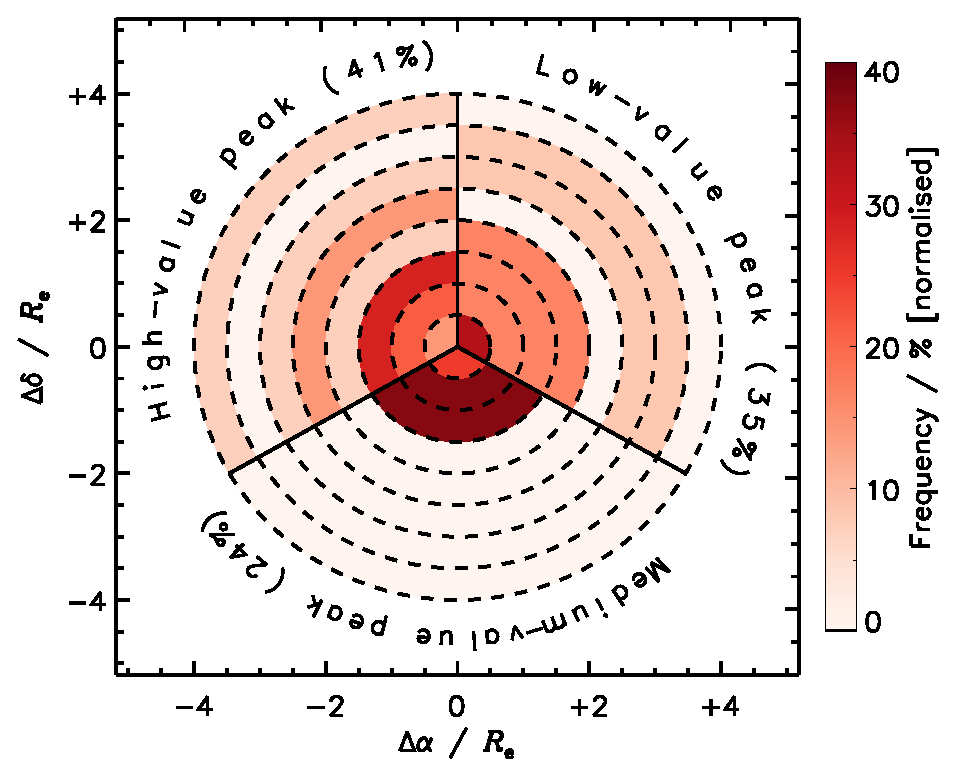
\includegraphics[width=1.2\columnwidth]{proximity}
    \caption{Radial distance of the $\sim60\%$ of ultra-red galaxies that show a positive over-density parameter to their closest global over-density peak.
    These peaks are divided into low, medium and high values (solid black lines) that are represented by three segments with radial offsets that increment by $0.5R_{\text{eff}}\approx2\arcmin$ (dashed black lines).
    The majority ($\approx60\%$) of over-dense ultra-red galaxies are located next to a medium- or high-value peak.
    Those nearest to a medium-value peak are all distributed within $<1.5R_{\text{eff}}\approx7\arcmin$ (or $3\,\text{Mpc}$ at $z\sim3$) of the peak position -- suggesting that these ultra-red galaxies may play a dominant role in such environments.
    On the other hand, only $\sim2/3$ of ultra-red galaxies that are nearest to a high-value peak are distributed within a similar scale and the remaining $\sim1/3$ are distributed as far out as $\approx4R_{\text{eff}}\approx20\arcmin$.
    A similar picture is seen for the $\approx33\%$ of over-dense ultra-red galaxies that are closest to a low-value peak, although a slight enhancement is seen within the inner-most radial bin.}
    \label{fig:proximity}
\end{figure*}

\subsection{Previously Identified Proto-Clusters}

A comprehensive review of previously identified/confirmed proto-clusters is given in \citet{casey16}, but we now briefly outline those found within some of the fields that we have analysed in this chapter.

\begin{itemize}
    \item A proto-cluster containing seven DSFGs at $z\sim2.5$ within the COSMOS field was serendipitously unveiled by \citet{casey15}.
    Situated in the centre and $\approx10\arcmin{}$ north of this over-density are the \urgs{} \mbox{S2COSMOSJ100025+022605} and \mbox{S2COSMOSJ100013+023429}, respectively.
    Although not officially catalogued as part of this proto-cluster, these \urgs{} have photometric redshifts of $\zphot{}=2.95^{+0.36}_{-0.30}$ and $\zphot{}=2.77^{+0.33}_{-0.29}$, respectively.
    Thus, it is not inconceivable that these two \urgs{} are members of this $z\sim2.5$ structure (rather than residing behind it).
    Interestingly, none of the catalogued members of this structure meet the strict ultra-red criteria.
    Furthermore, the environment around \mbox{S2COSMOSJ100025+022605} (at the heart this \citeauthor{casey15} structure) shows no particular over-/under-density of DSFGs compared to the field over the $\sim5\text{-}\text{arcmin}$ scales that we have examined.
    \item \citet{hung16} report a proto-cluster containing nine DSFGs at $z\approx2.1$ within the COSMOS field, $\approx10\,\arcmin{}$ south of the \citeauthor{casey15} structure.
    \item There is another confirmed proto-cluster within the COSMOS field containing four galaxies at $z\approx5.3$ \citep[the AzTEC-3 over-density ---][]{capak11, riechers10}.
    However, these galaxies are all contained within a single \scuba{} PSF, known as `COSMOS AzTEC-3'.
    \item Finally, there are five DSFGs comprising a proto-cluster in the GOODS-N field at $z=1.99$ \citep{blain04, chapman09}.
\end{itemize}

These previously identified proto-clusters provide a sample of $16$ spectroscopically confirmed DSFGs within $z\sim2\textrm{--}2.5$, which we used to measure the accuracy of the photometric redshift technique using the familiar expression $$\Delta z/(1+\zspec{}) \equiv (\zphot{} - \zspec{})/(1 + \zspec{}).$$
We found an accuracy and dispersion of $\mu_{|\Delta z|}\sim0.1\times(1+\zspec{})$ and $\sigma_{\Delta z}\sim0.1\times(1+\zspec{})$, respectively, re-iterating the predictive power of our photometric redshift algorithm, especially in this redshift interval.
These results are broadly consistent with those found in \citetalias{ivison16} and \citetalias{lewis17}.

Although this is only a small spectroscopic sample, these results are slightly more accurate, and reliable, than those achieved by \citet{michalowski17} for these same DSFGs, namely $\mu_{|\Delta z|}\sim0.2\times(1+\zspec{})$ and $\sigma_{\Delta z}\sim0.3\times(1+\zspec{})$, respectively.

\subsection{Associations Based on Photometric Redshifts}

The observed redshift ($1 + z_{\text{obs}}$) of a given galaxy (typically determined by frequency shifts in its observed spectrum, $\nu_{\text{rest}}/\nu_{\text{obs}}$) is composed of a (dominant) cosmological factor due to the expansion of space ($1 + z_{\text{cos}}$), a peculiar factor due to the velocity of that galaxy with respect to an observer (i.e. the Doppler effect, $1+z_{\text{pec}}$) and a gravitational factor due to the influence of strong gravitational fields in its vicinity ($1+z_{\text{grav}}$) as follows:
\begin{equation}
    \label{eq:redshift}
    \frac{\nu_{\text{rest}}}{\nu_{\text{obs}}} = (1+z_{\text{obs}})
    = (1+z_{\text{cos}}) (1+z_{\text{pec}}) (1+z_{\text{grav}}).
\end{equation}

Thus, testing whether a particular DSFG at a redshift $z$ is `associated' to another galaxy relies on being able to constrain their observed redshifts to within:
\begin{equation}
    \label{eq:vlos_assoc}
    |\Delta z|_{\text{assoc}} \lesssim \frac{2\sigma_{\text{los}}}{c}(1+z),
\end{equation}
\noindent
where $\sigma_{\text{los}}$ is line-of-sight velocity dispersion.
The typical velocity dispersion for (unvirialised) members of a distant ($z\gtrsim3$) proto-cluster is around $\sigma_{\text{los}}\approx500\,\text{km}\,\text{s}^{-1}$, but values as high as $\sigma_{\text{los}}\approx2{,}000\,\text{km}\,\text{s}^{-1}$ have been recorded \citep{venemans07, dey16}.
Finally, it is important to note that equation~(\ref{eq:vlos_assoc}) assumes that the two galaxies are at the same cosmological redshift ($z$) and neglects the effects from strong gravitational fields.
Furthermore, the factor of $2$ accounts for the fact that these two galaxies may be placed at opposing ends of a given structure when imaged.

In \citetalias{lewis17}, we associated galaxies within the same structure using an association threshold of $|\Delta z|_{\text{assoc}}\lesssim0.5$, which was based on the median photometric-redshift fitting errors for $z\sim3$ DSFGs using shallow FIR photometry.
However, not only is this threshold an order of magnitude greater than that expected from equation~(\ref{eq:vlos_assoc}) using the maximum velocity dispersion recorded in proto-clusters, this method also treated two DSFGs that were `associated' to a particular structure signposted by an \urg{} the same, regardless of how well their individual photometric redshifts were constrained.
% regardless of their individual redshift errors.

Thus, we have taken a different approach in this work and used the photometric redshift probability distributions and equation~(\ref{eq:vlos_assoc}) to assign each surrounding galaxy an `associated probability' ($\mathcal{P}_{\text{assoc}}$).
This probability was calculated by drawing $10{,}000$ redshift realisations from each photometric redshift distribution and determining the number of times that equation~(\ref{eq:vlos_assoc}) was satisfied.
Furthermore, we subsequently assigned each surrounding galaxy an `association weight' ($\mathcal{W}_{\text{assoc}}$), which was simply the association probability scaled by the fidelity of that particular galaxy.

For instance, the probability that one \urg{} is associated to another \urg{} (assuming that each have a photometric redshift of $\zphot=2.80\pm0.19$ and neglecting the $\sigma_{z}=0.14(1+z)\sim0.5$ intrinsic template SED scatter) to within $|\Delta z|_{\text{assoc}}\lesssim0.05$ is $\mathcal{P}_{\text{assoc}}\sim15\%$.
Furthermore, assuming that this \urg{} has a fidelity parameter of $\fidelity{}=0.8$, we would assign this particular surrounding galaxy an association weight of $\mathcal{W}_{\text{assoc}}\sim10\%$.

We were only able to associate (on average) $\approx1$ surrounding DSFG to an \urg{}, which was determined by summing the association weights from all of its surrounding galaxies within $\reff{}\sim5\arcmin{}$.
Interestingly, this is the same average number of associations achieved in \citetalias{lewis17}, which is perhaps indicative of the limitations with using FIR-based photometric redshifts.

\subsection{FIR Total Dust Masses and SFRs}

\begin{figure}
    \centering
    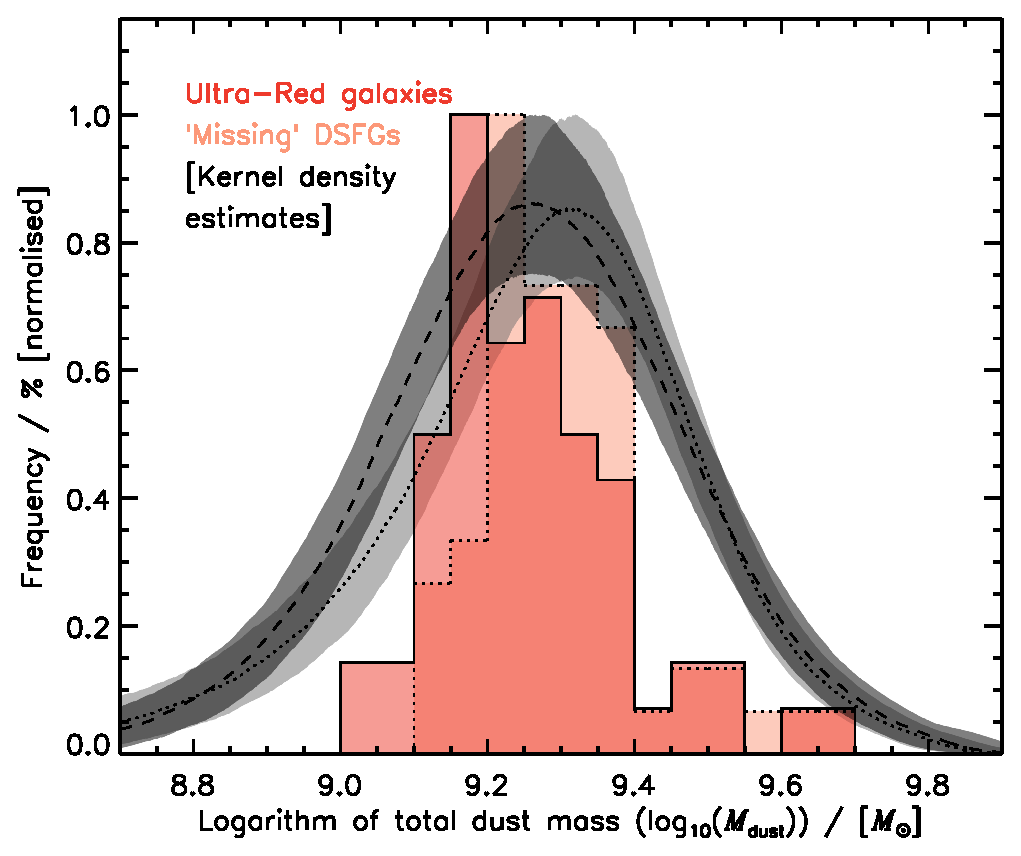
\includegraphics[width=\columnwidth]{dust_masses}\\\vspace{1em}
    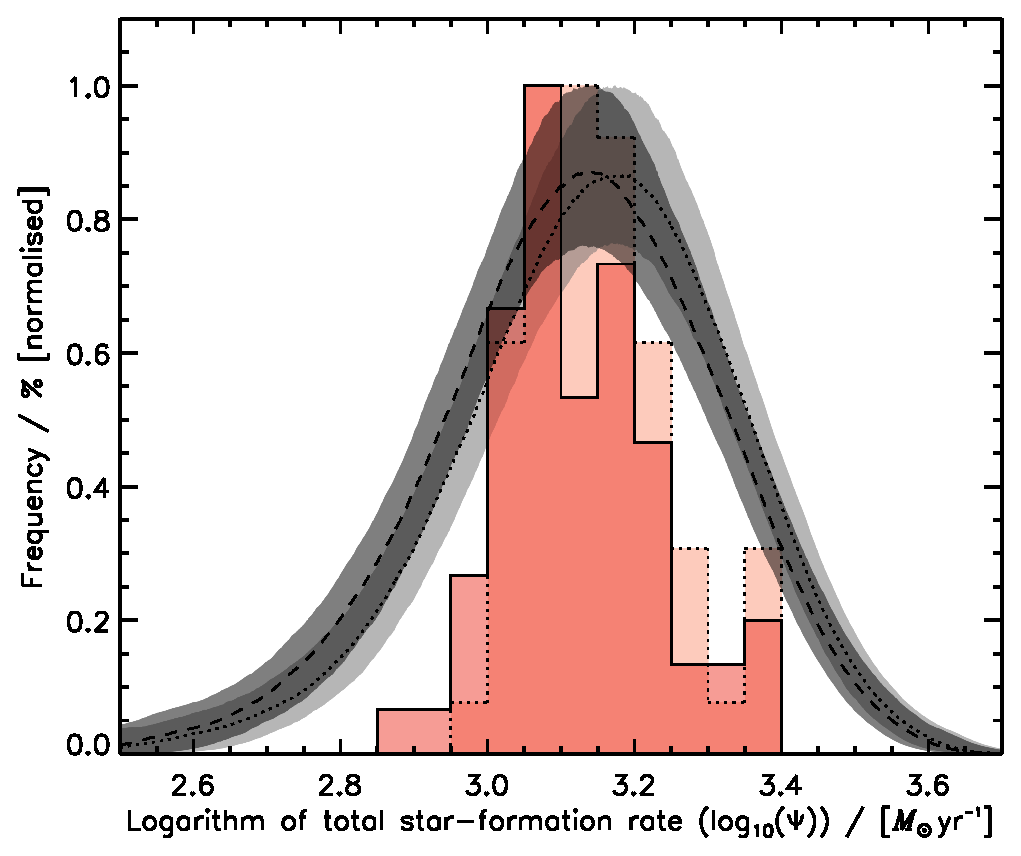
\includegraphics[width=\columnwidth]{star_formation_rates}
    \caption{\textbf{Top:} histogram of the total dust masses around ultra-red galaxies (red) and an arbitrarily normalised KDE (black), which was derived by averaging $1{,}000$ realisations of the total dust masses for the surrounding galaxies.
    Each surrounding DSFG within $\reff{}\approx5\arcmin{}$ has been weighted according to equation~(\ref{eq:vlos_assoc}).
    The total dust mass peaks at $\approx2\times10^{9}\,\msol{}$ -- equating to a molecular-gas reservoir of $\sim10^{11}\,\msol{}$, assuming a GDR of $\delta_{\text{GDR}}=100$.
    The dotted black lines show the effect of accounting for the `missing' DSFGs due to varying r.m.s.\ values around each ultra-red galaxy.
    These missing DSFGs increase the total dust mass in the environments of \urgs{} by a factor of $\sim1.25\times$.
    \textbf{Bottom:} histogram (red) and normalised KDE (black) of the total SFR for DSFGs in the $\reff{}\approx5\text{-}\text{arcmin}$ vicinity of ultra-red galaxies.
    Again, each SFR has been weighted accordingly and a contribution from the missing DSFGs has also been shown (dark grey).
    The peak of this distribution occurs at a total SFR of $\Psi\sim1{,}100\,\msol{}\,\text{yr}^{-1}$, which -- assuming a $100\text{-}\text{Myr}$ burst of star formation -- could easily result in a present-day structure with total stellar mass of $\mstars{}\sim10^{11}\,\msol{}$.}
    \label{fig:dust_masses}
\end{figure}

With a method for weighting the contributions from any surrounding DSFGs using equation~(\ref{eq:vlos_assoc}), we derived the total dust masses and total SFRs within the $5\text{-}\text{arcmin}$ environments around the \urgs{} catalogued in the S2CLS and S2COSMOS imaging surveys.
We show the results of these two properties in the top and bottom panels of Fig.~\ref{fig:dust_masses}, respectively, noting that these values exclude the contributions from the central \urgs{}.

The total dust masses peak at $\mdust{}\approx1.8\times10^{9}\,\msol{}$, whilst the total SFRs peak at $\Psi\approx1{,}400\,\msol{}\,\text{yr}^{-1}$.
These values are broadly consistent with those reported in \citetalias{lewis17}, namely $\mdust{}\sim1.7\times10^{9}\,\msol{}$ and $\Psi\approx1{,}100\,\msol{}\,\text{yr}^{-1}$, respectively, somewhat expected due to the same number of associated DSFGs.

As the expected number of galaxies within an aperture around any given DSFG varies -- reflective of the differing image r.m.s.\ values and/or edge effects -- we also computed the `missing' number of galaxies necessary to reconcile the shallowest regions with the deepest regions in an image.
We represented these missing DSFGs with the global photometric redshift distribution (see Fig.~\ref{fig:photoz_s2}), average dust masses of $1.2\times10^{9}\,\msol{}$ and average SFRs of $575\,\msol{}\,\text{yr}^{-1}$, with the latter two being computed using the method outlined in \citet{barlow04}.
However, the effect of including these missing galaxies was small, namely it increased the total dust masses and total SFRs by a factor of $\sim1.25\times$ to $\mdust{}\approx2.2\times10^{9}\,\msol{}$ and $\Psi\approx1{,}600\,\msol{}\,\text{yr}^{-1}$, respectively.

Finally, it is worth mentioning that total dust masses and total SFRs computed via this method converged as the association weight of surrounding galaxies tended to zero ($\mathcal{W}_{\text{assoc}}\to0$), suggesting that including all of the surrounding galaxies in this calculation was reasonable.

\section{Optical/NIR Analysis}

\begin{landscape}
\begin{table}
    \caption{Ultra-Red galaxies and their environmental properties.}
    \label{tab:fir_nir_environments}
    \begin{tabular}{l c c c c c c c c c c c c}
        \hline
        IAU & Field & $z$ & $P_{\text{UR}}$ & $\sum\fidelity{}$ & $\delta_{\reff{}}^{\dagger}$ & $\sum\mathcal{P}_{\text{assoc}}^{\dagger}$ & $\log_{10}(\mdust{})^{\dagger}$ & $\log_{10}(\Psi)^{\dagger}$ & $\sum\mathcal{P}_{\text{assoc}}$ & $\delta_{\reff{}}$ & $\log_{10}(\mstars{})$\\
        & & & $\%$ & & & & $[\msol{}]$ & $[\msol{}\,\text{yr}^{-1}]$ & & & $[\msol{}]$\\
        & & \multicolumn{7}{c}{\dotfill\,\textbf{FIR}\,\dotfill} & \multicolumn{3}{c}{\dotfill\,\textbf{Optical/NIR}\,\dotfill}\\
        \hline
        S2COSMOSJ100249+023255 & COSMOS & $3.72^{+0.35}_{-0.33}$ & $91.1^{+0.3}_{-0.3}$ & $8.7^{+4.0}_{-2.8}$ & $+0.3^{+0.6}_{-0.4}$ & $0.2^{+0.1}_{-0.1}$ & $9.5^{+0.1}_{-0.1}$ & $3.4^{+0.1}_{-0.1}$ & $10.5^{+1.0}_{-1.3}$ & $-0.1^{+0.3}_{-0.2}$ & 11.2\\
        S2COSMOSJ095748+015843 & COSMOS & $3.25^{+0.40}_{-0.34}$ & $70.9^{+0.3}_{-0.3}$ & $4.8^{+3.3}_{-2.1}$ & $-0.2^{+0.6}_{-0.4}$ & $0.3^{+0.2}_{-0.1}$ & $9.3^{+0.1}_{-0.1}$ & $3.1^{+0.1}_{-0.1}$ & $22.3^{+2.2}_{-2.6}$ & $+0.1^{+0.3}_{-0.2}$ & 11.5\\
        S2CLSJ021620-045054 & UDS & $2.85^{+0.32}_{-0.28}$ & $70.7^{+0.3}_{-0.3}$ & $16.7^{+4.9}_{-3.9}$ & $-0.4^{+0.2}_{-0.1}$ & $0.6^{+0.2}_{-0.2}$ & $9.2^{+0.2}_{-0.2}$ & $3.1^{+0.2}_{-0.2}$ & $15.3^{+2.7}_{-1.4}$ & $-0.1^{+0.1}_{-0.1}$ & 11.5\\
        S2COSMOSJ100209+023633 & COSMOS & $3.22^{+0.36}_{-0.32}$ & $68.1^{+0.3}_{-0.3}$ & $13.5^{+4.7}_{-3.6}$ & $+0.9^{+0.7}_{-0.5}$ & $0.4^{+0.1}_{-0.1}$ & $9.3^{+0.1}_{-0.1}$ & $3.2^{+0.1}_{-0.1}$ & $29.0^{+2.0}_{-3.6}$ & $+0.3^{+0.5}_{-0.3}$ & 11.6\\
        S2COSMOSJ100323+023352 & COSMOS & $2.73^{+0.27}_{-0.26}$ & $67.9^{+0.3}_{-0.3}$ & $1.0^{+2.3}_{-0.8}$ & $-0.8^{+0.4}_{-0.1}$ & $0.3^{+0.8}_{-0.3}$ & $9.3^{+0.1}_{-0.1}$ & $3.2^{+0.1}_{-0.1}$ & --- & --- & ---\\
        S2COSMOSJ100235+024731 & COSMOS & $2.88^{+0.35}_{-0.29}$ & $65.4^{+0.3}_{-0.3}$ & $9.9^{+4.2}_{-3.1}$ & $+0.6^{+0.7}_{-0.5}$ & $0.6^{+0.2}_{-0.2}$ & $9.2^{+0.2}_{-0.2}$ & $3.1^{+0.2}_{-0.2}$ & $34.1^{+3.1}_{-3.9}$ & $+0.2^{+0.4}_{-0.3}$ & 11.7\\
        S2COSMOSJ095931+023043 & COSMOS & $2.87^{+0.28}_{-0.26}$ & $64.6^{+0.3}_{-0.3}$ & $9.6^{+4.1}_{-3.0}$ & $+0.1^{+0.5}_{-0.3}$ & $0.4^{+0.2}_{-0.1}$ & $9.3^{+0.1}_{-0.1}$ & $3.1^{+0.1}_{-0.1}$ & $28.6^{+2.4}_{-3.9}$ & $+0.2^{+0.5}_{-0.3}$ & 11.6\\
        S2CLSJ021631-052622 & UDS & $2.79^{+0.27}_{-0.25}$ & $61.8^{+0.2}_{-0.2}$ & $16.5^{+5.1}_{-4.0}$ & $-0.1^{+0.3}_{-0.2}$ & $0.6^{+0.2}_{-0.1}$ & $9.3^{+0.1}_{-0.1}$ & $3.2^{+0.1}_{-0.1}$ & --- & --- & ---\\
        S2COSMOSJ100257+014257 & COSMOS & $2.58^{+0.30}_{-0.27}$ & $60.2^{+0.2}_{-0.2}$ & $5.0^{+3.4}_{-2.1}$ & $-0.1^{+0.6}_{-0.4}$ & $0.6^{+0.4}_{-0.2}$ & $9.2^{+0.1}_{-0.2}$ & $3.1^{+0.1}_{-0.2}$ & --- & --- & ---\\
        S2COSMOSJ100115+024257 & COSMOS & $2.44^{+0.23}_{-0.23}$ & $56.5^{+0.2}_{-0.2}$ & $6.9^{+3.7}_{-2.5}$ & $-0.2^{+0.4}_{-0.3}$ & $0.6^{+0.3}_{-0.2}$ & $9.3^{+0.1}_{-0.1}$ & $3.2^{+0.1}_{-0.1}$ & $52.8^{+3.6}_{-4.3}$ & $+0.2^{+0.4}_{-0.3}$ & 12.0\\
        S2COSMOSJ095738+015813 & COSMOS & $3.02^{+0.35}_{-0.32}$ & $56.4^{+0.2}_{-0.2}$ & $4.9^{+3.3}_{-2.1}$ & $+1.4^{+1.6}_{-1.0}$ & $0.5^{+0.3}_{-0.2}$ & $9.3^{+0.1}_{-0.1}$ & $3.1^{+0.1}_{-0.1}$ & $19.8^{+2.6}_{-3.5}$ & $-0.2^{+0.3}_{-0.2}$ & 11.5\\
        S2COSMOSJ100140+023011 & COSMOS & $2.76^{+0.44}_{-0.38}$ & $55.2^{+0.2}_{-0.2}$ & $4.9^{+3.3}_{-2.1}$ & $-0.4^{+0.4}_{-0.3}$ & $0.4^{+0.3}_{-0.2}$ & $9.2^{+0.2}_{-0.2}$ & $3.0^{+0.2}_{-0.2}$ & $46.9^{+2.5}_{-4.3}$ & $+0.3^{+0.5}_{-0.3}$ & 11.9\\
        S2COSMOSJ100142+014033 & COSMOS & $2.87^{+0.30}_{-0.27}$ & $52.5^{+0.2}_{-0.2}$ & $6.9^{+3.7}_{-2.5}$ & $+0.1^{+0.6}_{-0.4}$ & $0.6^{+0.3}_{-0.2}$ & $9.4^{+0.1}_{-0.1}$ & $3.2^{+0.1}_{-0.1}$ & $26.4^{+2.6}_{-4.8}$ & $-0.2^{+0.4}_{-0.2}$ & 11.6\\
        S2CLSJ141715+523630 & EGS & $2.70^{+0.30}_{-0.27}$ & $51.5^{+0.2}_{-0.2}$ & $10.5^{+4.2}_{-3.1}$ & $+0.3^{+0.5}_{-0.4}$ & $0.6^{+0.3}_{-0.2}$ & $9.3^{+0.1}_{-0.2}$ & $3.1^{+0.1}_{-0.2}$ & --- & --- & ---\\
        S2CLSJ021730-045936 & UDS & $2.82^{+0.25}_{-0.24}$ & $51.4^{+0.2}_{-0.2}$ & $18.9^{+5.3}_{-4.2}$ & $-0.0^{+0.3}_{-0.2}$ & $0.5^{+0.1}_{-0.1}$ & $9.3^{+0.1}_{-0.1}$ & $3.2^{+0.1}_{-0.1}$ & $21.8^{+2.0}_{-2.4}$ & $-0.1^{+0.1}_{-0.1}$ & 11.5\\
        S2CLSJ104456+584959 & LHN & $2.82^{+0.31}_{-0.29}$ & $51.3^{+0.2}_{-0.2}$ & $9.0^{+3.8}_{-2.8}$ & $-0.2^{+0.4}_{-0.3}$ & $0.3^{+0.1}_{-0.1}$ & $9.4^{+0.1}_{-0.1}$ & $3.1^{+0.1}_{-0.1}$ & --- & --- & ---\\
        S2CLSJ021940-045618 & UDS & $2.09^{+0.21}_{-0.23}$ & $51.0^{+0.2}_{-0.2}$ & $20.2^{+5.4}_{-4.4}$ & $+0.2^{+0.3}_{-0.3}$ & $1.0^{+0.3}_{-0.2}$ & $9.2^{+0.1}_{-0.2}$ & $3.1^{+0.1}_{-0.2}$ & --- & --- & ---\\
        S2COSMOSJ100207+024137 & COSMOS & $2.55^{+0.30}_{-0.28}$ & $50.6^{+0.2}_{-0.2}$ & $10.6^{+4.3}_{-3.2}$ & $+0.6^{+0.7}_{-0.5}$ & $0.7^{+0.3}_{-0.2}$ & $9.3^{+0.1}_{-0.2}$ & $3.1^{+0.1}_{-0.2}$ & $45.5^{+4.3}_{-3.8}$ & $+0.2^{+0.5}_{-0.3}$ & 11.9\\
        S2CLSJ021744-052008 & UDS & $3.20^{+0.36}_{-0.28}$ & $50.4^{+0.2}_{-0.2}$ & $20.8^{+5.5}_{-4.4}$ & $+0.0^{+0.3}_{-0.2}$ & $0.6^{+0.2}_{-0.1}$ & $9.4^{+0.2}_{-0.2}$ & $3.2^{+0.2}_{-0.1}$ & $12.6^{+1.1}_{-1.4}$ & $-0.0^{+0.1}_{-0.1}$ & 11.3\\
        S2COSMOSJ095821+015937 & COSMOS & $3.01^{+0.38}_{-0.30}$ & $50.2^{+0.2}_{-0.2}$ & $7.7^{+3.8}_{-2.7}$ & $+0.1^{+0.5}_{-0.4}$ & $0.5^{+0.2}_{-0.2}$ & $9.2^{+0.2}_{-0.2}$ & $3.1^{+0.2}_{-0.2}$ & $33.7^{+2.6}_{-3.9}$ & $+0.2^{+0.4}_{-0.2}$ & 11.8\\
        S2COSMOSJ100136+021109 & COSMOS & $2.79^{+0.27}_{-0.24}$ & $49.0^{+0.2}_{-0.2}$ & $17.5^{+5.2}_{-4.1}$ & $+0.2^{+0.3}_{-0.3}$ & $0.9^{+0.3}_{-0.2}$ & $9.3^{+0.2}_{-0.2}$ & $3.2^{+0.2}_{-0.1}$ & $38.1^{+3.2}_{-4.9}$ & $+0.3^{+0.5}_{-0.3}$ & 11.8\\
        S2COSMOSJ100153+021941 & COSMOS & $2.47^{+0.26}_{-0.25}$ & $48.1^{+0.2}_{-0.2}$ & $18.4^{+5.3}_{-4.2}$ & $+0.5^{+0.4}_{-0.3}$ & $0.9^{+0.3}_{-0.2}$ & $9.2^{+0.2}_{-0.2}$ & $3.1^{+0.2}_{-0.2}$ & $33.0^{+2.7}_{-5.8}$ & $+0.1^{+0.4}_{-0.2}$ & 11.8\\
        S2COSMOSJ100059+013307 & COSMOS & $4.93^{+0.76}_{-0.45}$ & $48.0^{+0.2}_{-0.2}$ & $4.9^{+3.3}_{-2.1}$ & $+0.7^{+1.1}_{-0.8}$ & $0.1^{+0.1}_{-0.0}$ & $9.7^{+0.1}_{-0.1}$ & $3.4^{+0.1}_{-0.1}$ & --- & --- & ---\\
        S2COSMOSJ100317+024944 & COSMOS & $2.75^{+0.26}_{-0.25}$ & $47.1^{+0.2}_{-0.2}$ & $3.0^{+2.9}_{-1.6}$ & $+0.4^{+1.3}_{-0.8}$ & $0.8^{+0.7}_{-0.4}$ & $9.4^{+0.1}_{-0.1}$ & $3.3^{+0.1}_{-0.1}$ & --- & --- & ---\\
        S2COSMOSJ100025+022605 & COSMOS & $2.95^{+0.36}_{-0.30}$ & $47.1^{+0.2}_{-0.2}$ & $35.3^{+6.9}_{-5.9}$ & $-0.1^{+0.2}_{-0.2}$ & $1.0^{+0.2}_{-0.2}$ & $9.3^{+0.2}_{-0.2}$ & $3.2^{+0.2}_{-0.2}$ & $27.8^{+2.3}_{-3.7}$ & $+0.0^{+0.4}_{-0.2}$ & 11.7\\
        S2CLSJ021556-052106 & UDS & $2.46^{+0.21}_{-0.20}$ & $46.6^{+0.2}_{-0.2}$ & $17.4^{+5.0}_{-4.0}$ & $+0.3^{+0.4}_{-0.3}$ & $0.8^{+0.2}_{-0.2}$ & $9.4^{+0.2}_{-0.1}$ & $3.3^{+0.1}_{-0.1}$ & --- & --- & ---\\
        S2CLSJ021702-052718 & UDS & $2.22^{+0.31}_{-0.33}$ & $46.3^{+0.2}_{-0.2}$ & $21.0^{+5.4}_{-4.3}$ & $+0.1^{+0.3}_{-0.2}$ & $0.9^{+0.2}_{-0.2}$ & $9.1^{+0.2}_{-0.2}$ & $3.0^{+0.2}_{-0.2}$ & $38.0^{+3.2}_{-3.1}$ & $-0.1^{+0.1}_{-0.1}$ & 11.9\\
        S2COSMOSJ095946+015715 & COSMOS & $3.08^{+0.34}_{-0.29}$ & $46.2^{+0.2}_{-0.2}$ & $12.7^{+4.6}_{-3.5}$ & $+0.3^{+0.5}_{-0.4}$ & $0.6^{+0.2}_{-0.2}$ & $9.3^{+0.2}_{-0.1}$ & $3.2^{+0.1}_{-0.1}$ & $29.5^{+2.3}_{-2.7}$ & $-0.0^{+0.3}_{-0.2}$ & 11.6\\
        S2CLSJ021724-044030 & UDS & $2.65^{+0.31}_{-0.28}$ & $46.1^{+0.2}_{-0.2}$ & $13.9^{+4.6}_{-3.5}$ & $-0.2^{+0.3}_{-0.2}$ & $0.7^{+0.2}_{-0.2}$ & $9.2^{+0.2}_{-0.2}$ & $3.1^{+0.2}_{-0.2}$ & $17.5^{+2.8}_{-2.3}$ & $-0.1^{+0.1}_{-0.1}$ & 11.5\\
        S2CLSJ123633+621408 & GOODS-N & $2.97^{+0.25}_{-0.23}$ & $45.6^{+0.2}_{-0.2}$ & $23.6^{+5.7}_{-4.7}$ & $+0.4^{+0.3}_{-0.3}$ & $0.9^{+0.2}_{-0.2}$ & $9.4^{+0.1}_{-0.1}$ & $3.2^{+0.1}_{-0.1}$ & --- & --- & ---\\
        S2CLSJ021753-051100 & UDS & $2.61^{+0.27}_{-0.25}$ & $45.2^{+0.2}_{-0.2}$ & $28.4^{+6.2}_{-5.2}$ & $+0.4^{+0.3}_{-0.3}$ & $1.3^{+0.3}_{-0.2}$ & $9.3^{+0.2}_{-0.2}$ & $3.1^{+0.2}_{-0.2}$ & $33.5^{+3.3}_{-2.3}$ & $+0.0^{+0.1}_{-0.1}$ & 11.9\\
        S2COSMOSJ095715+022008 & COSMOS & $2.96^{+0.43}_{-0.44}$ & $45.2^{+0.2}_{-0.2}$ & $1.9^{+2.6}_{-1.3}$ & $+0.5^{+1.9}_{-1.0}$ & $0.4^{+0.6}_{-0.3}$ & $9.3^{+0.1}_{-0.2}$ & $3.2^{+0.1}_{-0.2}$ & $3.3^{+2.4}_{-3.6}$ & $-0.9^{+0.0}_{-0.0}$ & 10.9\\
        S2CLSJ021915-044408 & UDS & $2.38^{+0.24}_{-0.22}$ & $44.4^{+0.2}_{-0.2}$ & $16.2^{+5.0}_{-3.9}$ & $-0.2^{+0.3}_{-0.2}$ & $0.8^{+0.2}_{-0.2}$ & $9.3^{+0.1}_{-0.1}$ & $3.2^{+0.1}_{-0.1}$ & --- & --- & ---\\
        S2CLSJ021644-050222 & UDS & $2.57^{+0.22}_{-0.21}$ & $44.3^{+0.2}_{-0.2}$ & $21.8^{+5.6}_{-4.5}$ & $+0.1^{+0.3}_{-0.2}$ & $1.1^{+0.3}_{-0.2}$ & $9.4^{+0.1}_{-0.1}$ & $3.2^{+0.1}_{-0.1}$ & --- & --- & ---\\
        \hline\\
    \end{tabular}
\end{table}
\end{landscape}

\addtocounter{table}{-1}

\begin{landscape}
\begin{table}
    \caption{(Continued ...)}
    \begin{tabular}{l c c c c c c c c c c c c}
        \hline
        IAU & Field & $z$ & $P_{\text{UR}}$ & $\sum\fidelity{}$ & $\delta_{\reff{}}^{\dagger}$ & $\sum\mathcal{P}_{\text{assoc}}^{\dagger}$ & $\log_{10}(\mdust{})^{\dagger}$ & $\log_{10}(\Psi)^{\dagger}$ & $\sum\mathcal{P}_{\text{assoc}}$ & $\delta_{\reff{}}$ & $\log_{10}(\mstars{})$\\
        & & & $\%$ & & & & $[\msol{}]$ & $[\msol{}\,\text{yr}^{-1}]$ & & & $[\msol{}]$\\
        & & \multicolumn{7}{c}{\dotfill\,\textbf{FIR}\,\dotfill} & \multicolumn{3}{c}{\dotfill\,\textbf{Optical/NIR}\,\dotfill}\\
        \hline
        S2COSMOSJ095835+025327 & COSMOS & $2.63^{+0.28}_{-0.26}$ & $43.8^{+0.2}_{-0.2}$ & $2.9^{+2.8}_{-1.6}$ & $-0.6^{+0.4}_{-0.2}$ & $0.4^{+0.4}_{-0.2}$ & $9.3^{+0.1}_{-0.1}$ & $3.1^{+0.1}_{-0.1}$ & --- & --- & ---\\
        S2COSMOSJ095947+013659 & COSMOS & $2.70^{+0.31}_{-0.28}$ & $43.1^{+0.2}_{-0.2}$ & $5.9^{+3.5}_{-2.3}$ & $-0.1^{+0.5}_{-0.4}$ & $0.5^{+0.3}_{-0.2}$ & $9.2^{+0.2}_{-0.2}$ & $3.1^{+0.1}_{-0.2}$ & $22.3^{+2.8}_{-4.2}$ & $-0.1^{+0.4}_{-0.2}$ & 11.5\\
        S2COSMOSJ100013+023429 & COSMOS & $2.77^{+0.33}_{-0.29}$ & $42.6^{+0.2}_{-0.2}$ & $25.6^{+6.1}_{-5.0}$ & $+0.4^{+0.3}_{-0.3}$ & $1.1^{+0.3}_{-0.2}$ & $9.4^{+0.2}_{-0.1}$ & $3.2^{+0.2}_{-0.1}$ & $28.5^{+3.3}_{-3.7}$ & $+0.3^{+0.4}_{-0.3}$ & 11.6\\
        S2CLSJ021543-050050 & UDS & $2.42^{+0.32}_{-0.31}$ & $41.9^{+0.2}_{-0.2}$ & $11.2^{+4.3}_{-3.2}$ & $-0.1^{+0.3}_{-0.3}$ & $0.6^{+0.2}_{-0.2}$ & $9.2^{+0.2}_{-0.2}$ & $3.0^{+0.2}_{-0.2}$ & --- & --- & ---\\
        S2CLSJ021931-045826 & UDS & $2.83^{+0.36}_{-0.28}$ & $41.1^{+0.2}_{-0.2}$ & $23.1^{+5.8}_{-4.7}$ & $+0.3^{+0.3}_{-0.3}$ & $0.7^{+0.2}_{-0.1}$ & $9.2^{+0.2}_{-0.2}$ & $3.1^{+0.2}_{-0.2}$ & $18.6^{+2.1}_{-2.1}$ & $+0.0^{+0.1}_{-0.1}$ & 11.5\\
        S2CLSJ021756-045244 & UDS & $2.36^{+0.26}_{-0.24}$ & $41.0^{+0.2}_{-0.2}$ & $15.2^{+4.8}_{-3.8}$ & $-0.2^{+0.2}_{-0.2}$ & $0.6^{+0.2}_{-0.2}$ & $9.2^{+0.2}_{-0.2}$ & $3.0^{+0.1}_{-0.2}$ & $29.8^{+3.4}_{-3.2}$ & $+0.0^{+0.1}_{-0.1}$ & 11.7\\
        S2COSMOSJ100202+014453 & COSMOS & $3.19^{+0.36}_{-0.31}$ & $40.9^{+0.2}_{-0.2}$ & $6.7^{+3.6}_{-2.5}$ & $+0.0^{+0.5}_{-0.4}$ & $0.4^{+0.2}_{-0.1}$ & $9.3^{+0.1}_{-0.1}$ & $3.2^{+0.1}_{-0.1}$ & $10.2^{+2.0}_{-3.3}$ & $-0.3^{+0.3}_{-0.2}$ & 11.2\\
        S2CLSJ021833-052042 & UDS & $2.46^{+0.28}_{-0.27}$ & $40.7^{+0.2}_{-0.2}$ & $26.3^{+6.0}_{-4.9}$ & $+0.3^{+0.3}_{-0.3}$ & $1.2^{+0.3}_{-0.2}$ & $9.3^{+0.2}_{-0.2}$ & $3.1^{+0.2}_{-0.2}$ & $42.7^{+3.6}_{-2.7}$ & $+0.0^{+0.1}_{-0.1}$ & 11.9\\
        S2COSMOSJ100039+023843 & COSMOS & $2.63^{+0.35}_{-0.31}$ & $40.5^{+0.2}_{-0.2}$ & $15.7^{+5.0}_{-3.9}$ & $+0.2^{+0.4}_{-0.3}$ & $0.7^{+0.2}_{-0.2}$ & $9.2^{+0.2}_{-0.2}$ & $3.1^{+0.2}_{-0.2}$ & $25.6^{+3.1}_{-4.1}$ & $+0.0^{+0.4}_{-0.2}$ & 11.7\\
        S2COSMOSJ095829+025227 & COSMOS & $2.66^{+0.38}_{-0.33}$ & $40.3^{+0.2}_{-0.2}$ & $5.8^{+3.5}_{-2.3}$ & $-0.2^{+0.5}_{-0.3}$ & $0.5^{+0.3}_{-0.2}$ & $9.1^{+0.2}_{-0.2}$ & $3.0^{+0.1}_{-0.2}$ & --- & --- & ---\\
        S2COSMOSJ100340+023638 & COSMOS & $2.65^{+0.34}_{-0.37}$ & $39.6^{+0.2}_{-0.2}$ & $2.0^{+2.6}_{-1.3}$ & $+0.9^{+2.5}_{-1.2}$ & $0.9^{+1.1}_{-0.6}$ & $9.4^{+0.1}_{-0.2}$ & $3.2^{+0.1}_{-0.2}$ & --- & --- & ---\\
        S2COSMOSJ100242+021407 & COSMOS & $2.61^{+0.30}_{-0.26}$ & $39.5^{+0.2}_{-0.2}$ & $7.8^{+3.9}_{-2.7}$ & $-0.2^{+0.4}_{-0.3}$ & $0.5^{+0.3}_{-0.2}$ & $9.2^{+0.1}_{-0.2}$ & $3.1^{+0.1}_{-0.2}$ & $37.3^{+3.3}_{-4.4}$ & $+0.0^{+0.5}_{-0.2}$ & 11.8\\
        S2CLSJ021803-045526 & UDS & $2.87^{+0.27}_{-0.24}$ & $39.0^{+0.2}_{-0.2}$ & $20.7^{+5.4}_{-4.4}$ & $+0.0^{+0.3}_{-0.2}$ & $0.6^{+0.2}_{-0.1}$ & $9.5^{+0.1}_{-0.1}$ & $3.2^{+0.1}_{-0.1}$ & $18.8^{+1.7}_{-2.7}$ & $-0.0^{+0.1}_{-0.1}$ & 11.4\\
        S2CLSJ021921-052716 & UDS & $2.52^{+0.25}_{-0.23}$ & $38.8^{+0.2}_{-0.2}$ & $11.5^{+4.4}_{-3.3}$ & $+0.2^{+0.5}_{-0.3}$ & $0.6^{+0.2}_{-0.2}$ & $9.2^{+0.1}_{-0.1}$ & $3.1^{+0.1}_{-0.2}$ & --- & --- & ---\\
        S2COSMOSJ100252+024159 & COSMOS & $2.57^{+0.18}_{-0.18}$ & $38.7^{+0.2}_{-0.2}$ & $4.9^{+3.3}_{-2.1}$ & $-0.3^{+0.5}_{-0.3}$ & $0.6^{+0.4}_{-0.3}$ & $9.5^{+0.1}_{-0.1}$ & $3.4^{+0.1}_{-0.1}$ & $40.7^{+3.7}_{-4.4}$ & $-0.0^{+0.4}_{-0.2}$ & 11.8\\
        S2COSMOSJ100117+014247 & COSMOS & $2.90^{+0.26}_{-0.25}$ & $38.1^{+0.2}_{-0.2}$ & $8.7^{+4.0}_{-2.9}$ & $+0.2^{+0.5}_{-0.4}$ & $0.5^{+0.2}_{-0.2}$ & $9.4^{+0.1}_{-0.1}$ & $3.2^{+0.1}_{-0.1}$ & $38.8^{+3.7}_{-2.9}$ & $+0.1^{+0.4}_{-0.2}$ & 11.7\\
        S2CLSJ141557+520711 & EGS & $3.21^{+0.41}_{-0.31}$ & $37.9^{+0.2}_{-0.2}$ & $4.7^{+3.2}_{-2.0}$ & $-0.4^{+0.4}_{-0.2}$ & $0.1^{+0.1}_{-0.1}$ & $9.3^{+0.1}_{-0.1}$ & $3.2^{+0.1}_{-0.1}$ & --- & --- & ---\\
        S2COSMOSJ100252+022903 & COSMOS & $2.59^{+0.29}_{-0.27}$ & $37.7^{+0.2}_{-0.2}$ & $6.7^{+3.6}_{-2.5}$ & $-0.1^{+0.5}_{-0.3}$ & $0.6^{+0.3}_{-0.2}$ & $9.3^{+0.1}_{-0.1}$ & $3.1^{+0.1}_{-0.1}$ & $33.7^{+2.9}_{-4.1}$ & $-0.2^{+0.3}_{-0.2}$ & 11.8\\
        S2CLSJ021600-045938 & UDS & $2.34^{+0.28}_{-0.25}$ & $37.3^{+0.2}_{-0.2}$ & $19.8^{+5.3}_{-4.3}$ & $+0.1^{+0.3}_{-0.2}$ & $1.1^{+0.3}_{-0.2}$ & $9.3^{+0.2}_{-0.2}$ & $3.1^{+0.2}_{-0.2}$ & --- & --- & ---\\
        S2CLSJ021931-052156 & UDS & $2.44^{+0.32}_{-0.28}$ & $36.6^{+0.2}_{-0.2}$ & $11.3^{+4.3}_{-3.2}$ & $+0.4^{+0.5}_{-0.4}$ & $0.5^{+0.2}_{-0.1}$ & $9.1^{+0.2}_{-0.2}$ & $3.0^{+0.2}_{-0.2}$ & --- & --- & ---\\
        S2COSMOSJ095921+014737 & COSMOS & $2.78^{+0.30}_{-0.27}$ & $36.5^{+0.2}_{-0.2}$ & $4.7^{+3.2}_{-2.0}$ & $-0.3^{+0.5}_{-0.3}$ & $0.4^{+0.3}_{-0.2}$ & $9.2^{+0.1}_{-0.1}$ & $3.1^{+0.1}_{-0.1}$ & $35.0^{+2.3}_{-4.4}$ & $+0.0^{+0.4}_{-0.2}$ & 11.8\\
        S2COSMOSJ095759+014111 & COSMOS & $3.00^{+0.46}_{-0.36}$ & $36.4^{+0.2}_{-0.2}$ & $1.9^{+2.5}_{-1.2}$ & $-0.7^{+0.4}_{-0.2}$ & $0.3^{+0.4}_{-0.2}$ & $9.1^{+0.2}_{-0.2}$ & $3.0^{+0.2}_{-0.2}$ & $32.5^{+1.8}_{-3.8}$ & $+0.1^{+0.4}_{-0.2}$ & 11.7\\
        S2COSMOSJ095942+022937 & COSMOS & $3.27^{+0.34}_{-0.29}$ & $36.4^{+0.2}_{-0.2}$ & $12.5^{+4.5}_{-3.4}$ & $-0.1^{+0.3}_{-0.3}$ & $0.4^{+0.1}_{-0.1}$ & $9.4^{+0.1}_{-0.1}$ & $3.3^{+0.1}_{-0.1}$ & $20.3^{+1.8}_{-3.0}$ & $+0.3^{+0.5}_{-0.3}$ & 11.4\\
        S2CLSJ141826+524154 & EGS & $2.96^{+0.41}_{-0.31}$ & $36.0^{+0.2}_{-0.2}$ & $20.2^{+5.4}_{-4.4}$ & $+0.2^{+0.3}_{-0.3}$ & $0.6^{+0.2}_{-0.1}$ & $9.2^{+0.2}_{-0.2}$ & $3.1^{+0.2}_{-0.2}$ & --- & --- & ---\\
        S2COSMOSJ100141+022713 & COSMOS & $3.39^{+0.36}_{-0.32}$ & $36.0^{+0.2}_{-0.2}$ & $7.8^{+3.9}_{-2.7}$ & $-0.1^{+0.5}_{-0.3}$ & $0.3^{+0.1}_{-0.1}$ & $9.6^{+0.1}_{-0.1}$ & $3.4^{+0.1}_{-0.1}$ & $27.4^{+1.7}_{-2.5}$ & $+0.2^{+0.4}_{-0.2}$ & 11.7\\
        S2COSMOSJ095958+023459 & COSMOS & $2.98^{+0.37}_{-0.29}$ & $35.9^{+0.2}_{-0.2}$ & $20.5^{+5.5}_{-4.4}$ & $+0.5^{+0.4}_{-0.3}$ & $0.7^{+0.2}_{-0.1}$ & $9.2^{+0.2}_{-0.2}$ & $3.1^{+0.2}_{-0.2}$ & $22.7^{+2.7}_{-3.1}$ & $+0.2^{+0.5}_{-0.3}$ & 11.6\\
        S2COSMOSJ095922+025137 & COSMOS & $3.41^{+0.43}_{-0.35}$ & $35.9^{+0.2}_{-0.2}$ & $6.8^{+3.7}_{-2.5}$ & $+0.1^{+0.6}_{-0.4}$ & $0.3^{+0.2}_{-0.1}$ & $9.6^{+0.1}_{-0.1}$ & $3.3^{+0.1}_{-0.1}$ & --- & --- & ---\\
        S2CLSJ021805-051050 & UDS & $3.63^{+0.41}_{-0.32}$ & $35.5^{+0.2}_{-0.2}$ & $24.2^{+5.7}_{-4.7}$ & $+0.2^{+0.3}_{-0.2}$ & $0.4^{+0.1}_{-0.1}$ & $9.5^{+0.1}_{-0.1}$ & $3.3^{+0.2}_{-0.1}$ & $7.3^{+0.8}_{-0.6}$ & $+0.0^{+0.1}_{-0.1}$ & 11.1\\
        S2COSMOSJ095936+020419 & COSMOS & $2.44^{+0.26}_{-0.25}$ & $35.4^{+0.2}_{-0.2}$ & $7.8^{+3.8}_{-2.7}$ & $-0.2^{+0.4}_{-0.3}$ & $0.5^{+0.3}_{-0.2}$ & $9.2^{+0.2}_{-0.2}$ & $3.0^{+0.1}_{-0.2}$ & $37.2^{+2.5}_{-5.8}$ & $+0.1^{+0.4}_{-0.2}$ & 11.8\\
        S2CLSJ021822-050738 & UDS & $2.98^{+0.43}_{-0.32}$ & $35.2^{+0.2}_{-0.2}$ & $16.4^{+4.9}_{-3.8}$ & $-0.1^{+0.3}_{-0.2}$ & $0.5^{+0.2}_{-0.1}$ & $9.2^{+0.2}_{-0.2}$ & $3.0^{+0.2}_{-0.2}$ & $25.5^{+1.2}_{-2.3}$ & $-0.0^{+0.1}_{-0.1}$ & 11.6\\
        \hline
        \multicolumn{11}{l}{$^{\dagger}$ These parameters have been adjusted to account for `missing' DSFGs.}\\
        \multicolumn{11}{l}{\textbf{Note}. --- Ultra-Red galaxies are listed in decreasing order of ultra-red probability.}\\
    \end{tabular}
\end{table}
\end{landscape}

As discussed, \urgs{} appear to preferentially signpost over-densities of DSFGs and furthermore they appear to be situated near to the centres of medium-to-high-value over-density peaks.
Thus, this motivated us to examine the optical/NIR environments around these \urgs{}, with the aim to uncover any relationships that may, or may not, be present within such extreme environments at $z\gtrsim3$.
For instance, has the emergence of the red sequence taken place around \urgs{} at these redshifts yet?
Or, is their any dependence on the colour and/or stellar mass of galaxies as the radial distance from an \urg{} varies?
If these relationships are not uncovered, it may suggest that something is wrong with our understanding of the formation of massive galaxies at high redshift and the role that they play in the assembly of large structure.

\subsection{Optical/NIR Data Acquisition}

To answer these questions, we made use of publicly available, multi-wavelength catalogues covering the COSMOS\footnote{%
    \url{ftp://ftp.iap.fr/pub/from_users/hjmcc/COSMOS2015/COSMOS2015_Laigle+_v1.1.fits.gz}.}
 \citep{mccracken12, laigle16} and UDS\footnote{%
    \url{http://www.nottingham.ac.uk/~ppzoa/cls/UDS_DR8_forS2CLS_v4.dat.fits}.}
fields (Almaini et al., in prep.).
Although such catalogues do exist for the EGS and GOODS-N fields, their coverage does not include the regions occupied by the \urgs{} presented within this chapter.
As for the remaining fields, to the best of our knowledge, there are no available optical/NIR data.

The catalogue for the COSMOS field contains $606{,}887$ sources within an area of $\mathcal{A}\approx1.70\,\deg^2$ that comprises the UltraVISTA-\textsc{dr}2 region.
The catalogue for the UDS field contains $184{,}439$ sources detected over an area of $\mathcal{A}\approx0.77\,\deg^2$ that comprises the 8\textsuperscript{th} release \citep{hartley13} of the United Kingdom IR Telescope (UKIRT) IR Deep Sky Survey \citep[UKIDSS ---][]{lawrence07}.
Therefore, the surveyed area for both of these fields is slightly smaller than that surveyed by \scuba{}.
Hence, although there are $59$ \urgs{} within the COSMOS and UDS fields, there is only suitable optical/NIR coverage for $42$ \urgs{}; $30$ from the COSMOS field and $12$ from the UDS field.

For both of the fields, the photometric redshifts contained within the catalogues were computed using a $\chi^2$-minimisation code \citep{arnouts99} over a redshift grid of $0<\zphot{}<6$ down to a resolution of $\delta \zphot{}= 0.01$.
The implementation of this code used a combination of template SEDs (representing spiral, elliptical and young, blue star-forming galaxies), appropriately handled galactic dust extinction and was found to produce an intrinsic scatter of $\sigma_{\Delta z}=0.021(1+z)$ at $z>3$ -- far better than that achieved with the FIR template SEDs adopted here.
However, over $z\sim0\text{--}3$ the median upper and lower fitting uncertainties for these galaxies increases by a factor of $\sim5\times$ to $\sigma^{+}_{\znir{}}=0.11$ and $\sigma^{-}_{\znir{}}=0.23$, respectively, which dwarfs this intrinsic scatter.
We modelled each photometric redshift in the catalogue using a split-normal distribution defined as:
\begin{equation}
    \label{eq:split_normal}
    P =
    A\exp\begin{cases}
        -(\zphot{} - \znir{})^2/2({\sigma^{+}_{\znir{}}})^{2} & \text{if }\zphot{}>\znir{}\\
        -(\zphot{} - \znir{})^2/2({\sigma^{-}_{\znir{}}})^{2} & \text{otherwise},
    % P\left(\zphot{}, \znir{}, {\sigma^{+}_{\znir{}}},{\sigma^{-}_{\znir{}}}\right) =
    % A\exp\begin{cases}
    %     -(\zphot{} - \znir{})^2/2({\sigma^{+}_{\znir{}}})^{2} & \text{if }\zphot{}>\znir{}\\
    %     -(\zphot{} - \znir{})^2/2({\sigma^{-}_{\znir{}}})^{2} & \text{otherwise},
    \end{cases}
\end{equation}
where $A=\sqrt{2/\pi}/(\sigma^{+}_{\znir{}}+\sigma^{-}_{\znir{}})$ integral normalises this distribution and $\zphot{}$ is the redshift grid covering $0<\zphot{}<10$ down to a resolution of $\delta \zphot{}= 0.01$, i.e.\ mimicking that used for DSFGs in \citetalias{ivison16}, \citetalias{lewis17} and here.

These catalogues also provide absolute magnitudes ($M$) and stellar masses ($\mstars{}$).
The former were either taken directly from the best-fitting, rest-frame template SED, or $K$-corrected from the apparent magnitude ($m$) measured through the passband closest to $\lambda_{M}(1+z)$.
% \footnote{%
%     For instance, the $B$-band (at $\lambda_{M}=4{,}458.3\,\angstrom{}$) absolute magnitude would be calculated from the $H$-band (at $\lambda_{m}=16{,}453.4\,\angstrom{}$) apparent magnitude at $z=3$.
% }.
Stellar masses were typically derived by scaling (in the observed frame) large samples of synthetic spectra to the $K$-band apparent magnitude and taking the resulting modal (or best-fit) stellar mass of these spectra \citep[e.g.][]{mortlock13, mortlock15}.

LBGs around \urgs{} at $z\sim3$ should have limited-to-no data at wavelengths shorter than the central wavelength of $U$/$B$ bands due to the Lyman-$\alpha$ break at $1{,}216\,\angstrom{}$ causing them to `drop-out' of these passbands.
Thus, in order to ensure that the LBGs used in this analysis had \emph{robust} stellar mass and/or absolute magnitude estimates, we required that their detected $K$-band photometry was below the $(3\text{--}5)\text{-}\sigma_{K}$ limiting magnitude.
To further increase the completeness of this sample, we also required that their photometric redshifts were `satisfactory' (i.e.\ consistent with having a galaxy-shaped SED and a suitable $\chi^2$ value) and that their stellar masses were above $\mstars{}>10^{9}\,\msol{}$.

\begin{table*}
    \caption{COSMOS and UDS catalogue flags.}
    \label{tab:nir_catalogue_flags}
    \begin{tabular}{ccccl}
        \hline
        FITS field name & Value & FITS field name & Value & Description \\
        \hline
        \multicolumn{2}{c}{\dotfill\,\textbf{COSMOS}\dotfill} & \multicolumn{2}{c}{\dotfill\,\textbf{UDS}\dotfill}\\
        \texttt{TYPE} & $0$ & \texttt{Basic galaxy catalogue} & $\text{T}$ & Galaxy SED shape\\
        \texttt{ZPDF} & $>0$ & \texttt{chisq\_at\_maxL} & $\leq15$ & Satisfactory $\zphot{}$\\
        \texttt{Ksw\_MAG\_APER2} & $<24.5$ & \texttt{MAG\_APER\_K\_2.0} & $<24.6$ & $K$-Band cut\\
        \texttt{MASS\_BEST} &  $>9$ & \texttt{Bestfit\_Mass} &  $>9$ & Stellar-Mass cut\\
        \texttt{FLAG\_HJMCC} & $0$ & \textemdash & & UltraVISTA-\textsc{dr}2\\
        \hline
    \end{tabular}
\end{table*}

In Table~\ref{tab:nir_catalogue_flags}, we list the FITS binary field names and respective values necessary to implement these constraints on the catalogues, which reduce the number of sources in the COSMOS and UDS fields to $201{,}376$ and $61{,}750$, respectively.

\subsection{Robust Counterparts to DSFGs}

In order to determine which LBGs were associated to the environments around the \urgs{} presented here, we needed to first examine whether there were any underlying systematics between the FIR photometric redshifts ($\zfir{}$) and those provided in the catalogues discussed above ($\znir{}$).
To test for such systematics, we first matched all of the available DSFGs to their true (or `real') counterparts.

In this work, we adopted the likelihood ratio \citep[LR ---][]{chapin11, fleuren12, mcalpine13} method in order to locate potential counterparts to DSFGs, which is defined as:
\begin{equation}
    \label{eq:likelihood_ratio}
    \text{LR} = \frac{\text{Probability of being related}}{\text{Probability of being unrelated}} = \frac{f(r,\mathcal{R})q(K,z)}{n(K,z)},
\end{equation}
\noindent
where $q(K,z)$ and $n(K,z)$ are the $K$-band magnitude and redshift prior distributions of the real counterparts to DSFGs and background galaxies, respectively, and $$f(r,\mathcal{R})=\frac{1}{2\pi\mathcal{R}^2}\exp{(-r^2/\mathcal{R}^2)}$$ is a Gaussian weighting that takes into account the positional accuracy of a given DSFG.
The positional accuracy is capped above $\mathcal{R}\ge2\arcsec{}$ (i.e.\ the \scuba{} pixel scale) to avoid $\mathcal{R}\to0$ for those DSFGs detected at a high SNR.
Furthermore, as it is typically much greater than that deduced for optical/NIR galaxies (i.e.\ $\mathcal{R}<0.2\arcsec{}$), we do not add it (in quadrature) to the radial offset for DSFGs.

\begin{figure*}
    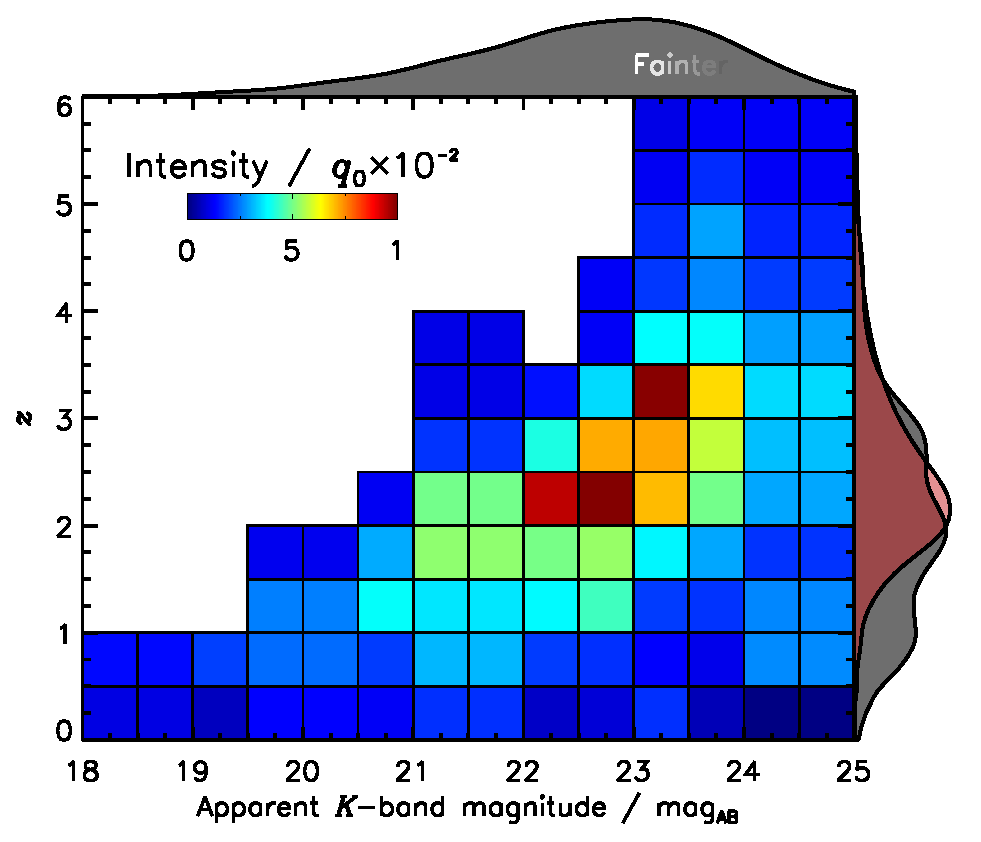
\includegraphics[width=1.075\columnwidth]{q_prior}
    \caption{The two-dimensional prior distribution for potential optical/NIR counterparts to $829$ DSFGs in the COSMOS field as a function of apparent $K$-band magnitude and redshift.
    This prior distribution was used to determine the LR that a given galaxy is the real counterpart to a given DSFG (see equation~(\ref{eq:likelihood_ratio})).
    We show the $K$-band magnitude distribution towards the top of the plot, which clearly shows that counterparts to DSFGs are faint, with $K$-band magnitudes peaking at $K\sim23\,\magab{}$ (or $S_{K}\sim2\times10^{-3}\,\millijanksy{}$).
    To the right, we show the photometric redshift distributions for the potential NIR counterparts (dark grey) and DSFGs (red, see \ref{fig:photoz_s2})
    The two distributions appear to be well matched around $z\approx2\text{--}3$, but seriously mismatched at $z\sim1$, which results in an extended tail of $K$-band magnitudes below $K\lesssim20\,\magab{}$.
    This mismatch is likely caused by the incorrect assignation of foreground galaxies to distant DSFGs.
    \textbf{Note.\ } Fainter apparent $K$-band magnitudes correspond to brighter galaxies.}
    \label{fig:q_prior}
\end{figure*}

We estimated the prior distributions of the counterparts and background galaxies as follows.

\begin{itemize}
    \item Firstly, we search for all galaxies within an $r_{\text{aper}}=8\text{-}\text{arcsec}$ radius of a given DSFG.
    Such a conservatively sized search radius accounts for the fact that some of the brightest DSFGs originally catalogued in the S2CLS UDS field were found to be offset by up to half of a \scuba{} PSF FWHM from their high-resolution counterparts detected with ALMA \citep[i.e.\ by as much as $\theta/2\approx8\arcsec{}$ ---][]{simpson15}.
    \item For any detected galaxies around a given DSFG, we select those that have apparent $K$-band magnitudes between $K'$ and $K'+\Delta K'$ (with $K'$ ranging from $K'=18\text{--}25\,\magab{}$ and $\Delta K'=0.5\,\magab{}$) and sum their respective photometric redshift distributions represented by equation~(\ref{eq:split_normal}).
    Performing this process for all DSFGs generates a two-dimensional `$total(K,z)$' image, which contains a contribution from the `background' galaxies and from the `real' counterparts, i.e.\ $$total(K,z)=background(K,z)+real(K,z).$$
    \item To determine the contribution from the background galaxies, the above steps are repeated but this time replacing the positions of the DSFGs with $10{,}000$ randomly generated positions.
    Normalising this background contribution by the area of the search radius, yields the prior distribution for the background galaxies, i.e.\ $$n(K,z) = \frac{background(K,z)}{\pi r_{\text{aper}} ^ 2}.$$
    \item Finally, the prior distribution for the real counterparts to the DSFGs can be determined by: $$q(K,z) = q_0\left(\frac{real(K,z)}{\sum_i real(K_i,z_i)}\right),$$
    where $q_0=69\pm4\%$ is a normalisation factor that estimates the probability of finding a real counterpart down to the $5\text{-}\sigma\lesssim24\,\magab{}$ survey limit, i.e.\ $\sim70\%$ of DSFGs have a real counterpart in the catalogues used here\footnote{$q_0$ was indirectly determined from a model fit of the form $(1-q_0f(r_{\text{aper}}))$ to the ratio of blank apertures (i.e.\ apertures containing no containing no galaxies) around DSFGs to those around random positions as a function of aperture radius from $r_{\text{aper}}=0\text{--}10\arcsec{}$.
        However, as we later normalise the LR by a factor dependent on the false-positive rate of `real' counterparts, determining $q_0$ is this way is not strictly necessary.}.
\end{itemize}

In Fig.~\ref{fig:q_prior}, we show $q(K,z)$ for the potential counterparts to $829$ DSFGs in the COSMOS field, noting that a similar prior distribution is derived for the UDS field.
Clearly the counterparts to DSFGs are faint, with typical $K$-band magnitudes of $K\sim23\,\magab{}$ (or equivalently $S_{K}\sim2\times10^{-3}\,\millijanksy{}$, i.e.\ a factor of $\gtrsim3{,}000\times$ fainter than at $850\,\micron{}$ for these DSFGs) -- similar to that seen in \citet{simpson14}.
Although the optical/NIR and FIR photometric redshift distribution appear to be well matched around $z\sim2\text{--}3$, there is a serious mismatch towards $z\sim1$, which results in an extended tail below $K\lesssim20\,\magab{}$.
This is likely caused by foreground (brighter) galaxies that have been incorrectly assigned as a real counterpart to a DSFG.
These incorrect assignations occur because either the real counterpart is too faint to be detected or (in extremely rare cases) outside of the $8\text{-}\text{arcsec}$ search radius.
As these incorrect matches will heavily skew any future analysis, they needed to be removed before comparing the FIR with the optical/NIR photometric redshift estimates.

To decide which counterparts to remove, we compared the LRs for the DSFGs already computed to those of a large control sample.
This large control sample was generated by calculating the LR for each DSFG after the centre of its search radius had be randomly tweaked.
The top-panel of Fig.~\ref{fig:likelihood_ratio} shows the distribution of LRs for DSFGs and this large control sample.
We highlight the LR that gives a false-positive rate of $10\%$, which was determined by integrating the tail of the control sample.
This false-positive rate corresponds to a LR of $\text{LR}=1.3$, above which only $\sim50\%$ of DSFGs have a real counterpart.

\begin{figure}
    \hspace{0.25em}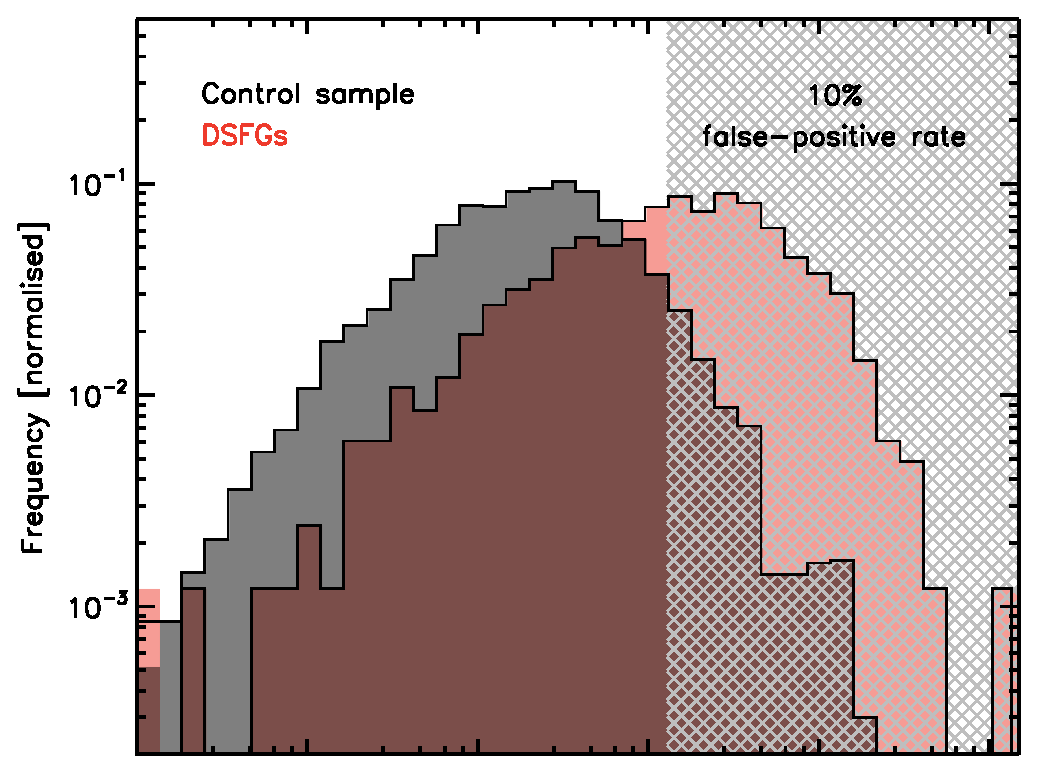
\includegraphics[width=0.99\columnwidth]{likelihood_ratio_false_positive}\\
    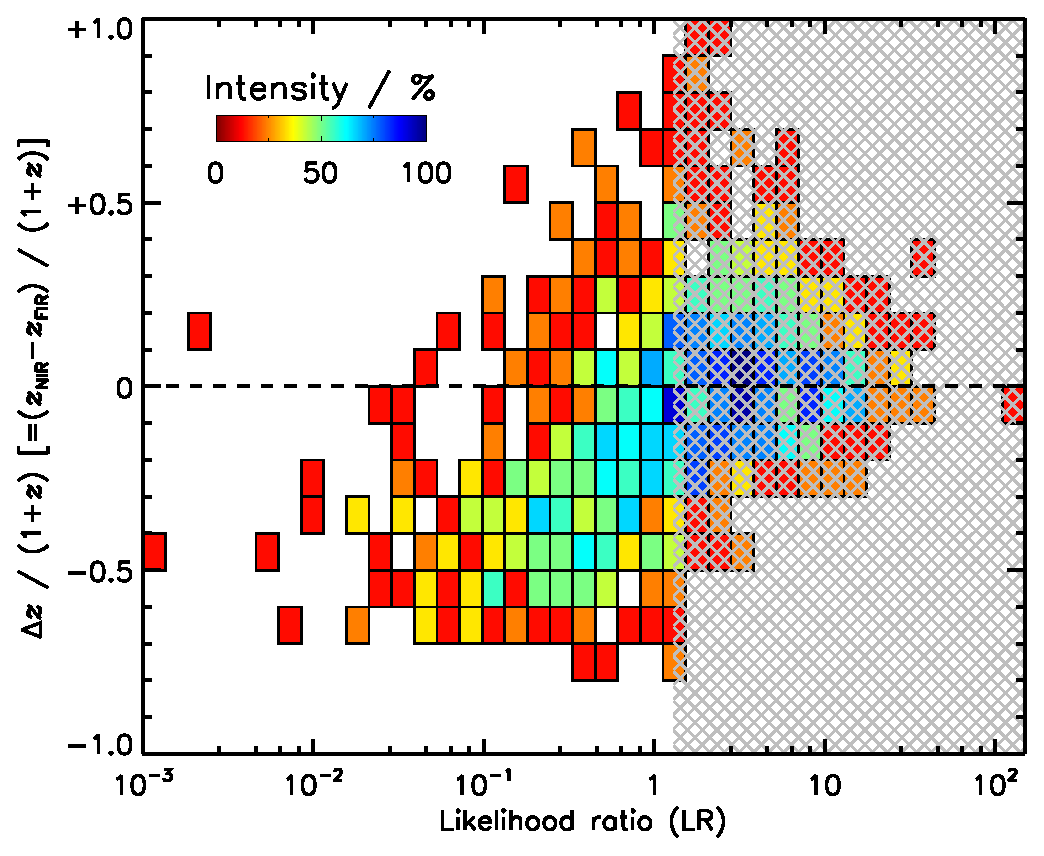
\includegraphics[width=\columnwidth]{likelihood_ratio}
    \caption{\textbf{Top:} histogram of the LRs for potential optical/NIR counterparts to DSFGs catalogued in the COSMOS field (black), which we compared to random positions (red).
    This comparison results in a false-positive rate of $10\%$ above a LR of $\text{LR}\gtrsim1.3$ (chequered light grey region).
    Only $50\%$ of DSFGs in the COSMOS field have a potential counter above this LR.
    \textbf{Bottom:} normalised difference, $(\znir-\zfir)/(1+\zfir)$, as a function of LR, between photometric redshifts determined using optical/NIR and FIR photometry.
    We obtain a LR-weighted mean and LR-weighted standard deviation of $\mu_{\Delta z}=+0.04(1+\zfir)$ and $\sigma_{\Delta z}=0.17(1+\zfir)$, respectively, for potential counterparts above $\text{LR}\gtrsim1.3$.
    Therefore, the FIR photometric redshifts presented here slightly under-estimate the optical/NIR photometric redshifts by $\mu_{\Delta z}=0.16$ at $z=3$, although this correction is uncertain to $\sigma_{\Delta z}=0.68$.
    Potential counterparts with LRs less than $\text{LR}<1$, have FIR photometric redshifts that are significantly higher than the optical/NIR ones -- suggesting that they are likely foreground galaxies.}
    \label{fig:likelihood_ratio}
\end{figure}

We then evaluated the normalised difference, $$\Delta z / (1+\zfir{}) \equiv (\znir{}-\zfir{})/(1+\zfir{}),$$ for each of these DSFG with a counterpart, which is shown in the bottom-panel of Fig.~\ref{fig:likelihood_ratio}.
We obtained a LR-weighted mean and LR-weighted standard deviation of $\mu_{\Delta z}=+0.04(1+\zfir{})$ and $\sigma_{\Delta z}=0.17(1+\zfir{})$, respectively, for these real counterparts.
This suggests that the FIR photometric redshifts presented here slightly under-estimate the optical/NIR photometric redshifts by $\mu_{\Delta z}=0.16$ at $z=3$, although this correction is intrinsically uncertain to $\sigma_{\Delta z}=0.68$.
Thus, before we evaluated the association probabilities of LBGs around \urgs{} using equation~(\ref{eq:vlos_assoc}), we shifted the FIR photometric redshift distribution of the \urgs{} by $+0.04(1+\zfir{})$, where $\zfir{}$ was taken from the peak of a given FIR photometric redshift distribution.

\subsection{Stellar Masses and Absolute Colours of LBGs}

With knowledge of how the FIR photometric redshifts correlate with the optical/NIR photometric redshifts, we examined the stellar masses ($\mstars{}$) and absolute $(M_B - M_I)$ colours of the LBGs surrounding the \urgs{} presented in this work.
To recap, there are $42$ \urgs{} with optical/NIR coverage, $30$ within the COSMOS field and $12$ within the UDS field.

At the positions of each of these \urgs{}, we extracted all of LBGs that lie within a radius of $\reff{}\approx5\arcmin{}$ and recorded their stellar masses, absolute $M_{B}$ and $M_{I}$ magnitudes, probability of being associated (to the `adjusted' FIR photometric redshift) using equation~(\ref{eq:vlos_assoc}) and radial distances to these positions.
We also generated a control sample for each \urg{} by extracting the same properties but at $100$ random positions, purposefully selected to avoid any overlap with the \urgs{}.

On average, there are $\approx28$ LBGs that are `associated' to given \urg{}, but this varies considerably from $\approx3\text{--}53$.
Although this only accounts for $\sim1\%$ of the optical/NIR galaxies that are typically within $\reff{}\approx5\arcmin{}$ of an \urg{}, this is still a factor of $\sim20\times$ the number of DSFGs that we were able to associate.
Thus, the contribution from surrounding LBGs is definitely not insignificant and, like for the associated DSFGs, is probably under-estimated here, too.

\subsubsection{Stellar Masses}

\begin{figure*}
    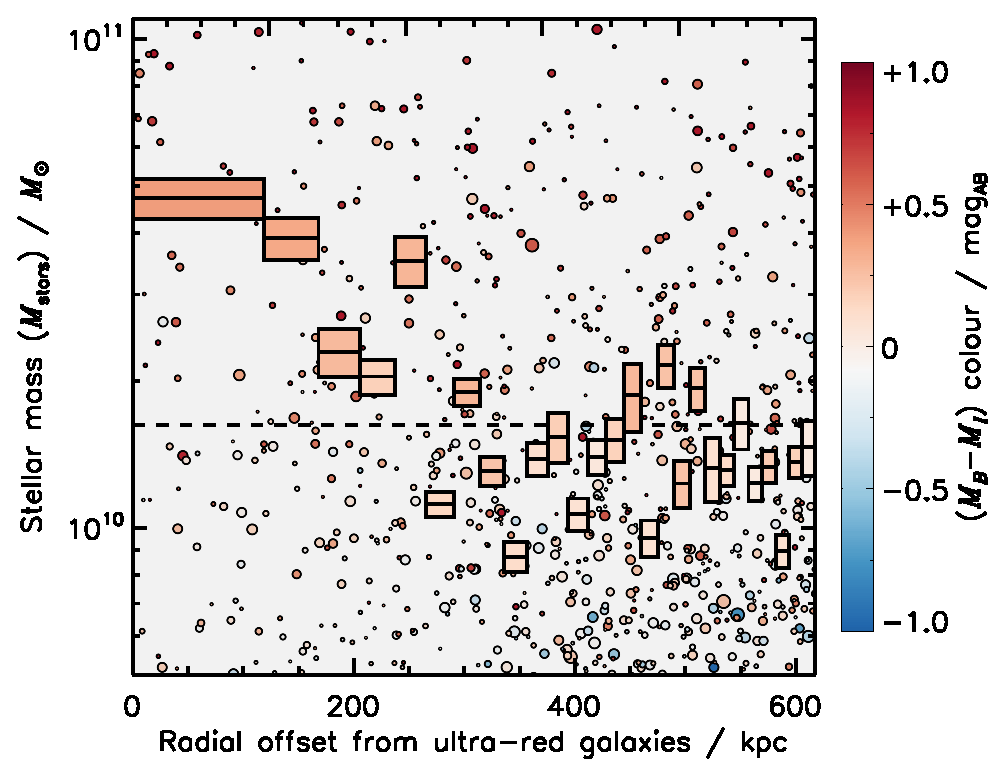
\includegraphics[width=1.25\columnwidth]{stellar_mass}\\
    \caption{Stellar mass and absolute colour variations of LBGs within $\lesssim500\,\kiloparsec{}$ of their respective central \urgs{}.
    Individual stellar mass measurements of the surrounding LBGs are represented as circles, colour-coded to represent their absolute ($M_{B}-M_{I}$) colour and scaled to represent their association probability to their respective \urgs{}.
    We show the average and standard error of the stellar mass within annuli of equal area.
    This figure illustrates that as the radial distance from an \urg{} increases out to $\sim400\,\kiloparsec{}$, the average stellar mass decreases by a factor of $\sim4\times$ to $\mstars{}=(1.1\pm0.1)\times10^{10}\,\msol{}$.
    This increasing average stellar mass with radius suggests that \urgs{} reside in over-dense environments.
    The black dashed line shows the typical annuli average stellar mass from the control sample $\mstars{}=(1.62\pm0.05)\times10^{10}\,\msol{}$.
    \textbf{Note.\ } This figure assumes that all \urgs{} are lying at $z\sim3$, where $1\arcmin{}$ corresponds to $\approx470\,\kiloparsec{}$.}
    \label{fig:stellar_mass}
\end{figure*}

In Fig.~\ref{fig:stellar_mass}, we show the stellar masses of the surrounding LBGs weighted by their association probability as a function of proper radial distance to their respective central \urgs{} (assuming that they reside at $z\sim3$).
The average stellar mass in annuli of equal area shows a slight decrease from $(4.7\pm0.4)\times10^{10}\,\msol{}$ at $\approx60\,\kiloparsec{}$ to $(1.1\pm0.1)\times10^{10}\,\msol{}$ at $\approx400\,\kiloparsec{}$.
Furthermore, the average $(M_{B}-M_{I})$-colour decreases from $0.57\pm0.02$ at $\approx60\,\kiloparsec{}$ to $0.28\pm0.02$ at $\approx400\,\kiloparsec{}$, too.
Although modest in size, these trends suggest that the \urgs{} are residing near the centres of potential wells extending over $\lesssim500\,\kiloparsec{}$ scales, and that these environmental factors are causing a factor of $\sim4\times$ and $\sim2\times$ increase in the stellar masses and colours of the surrounding LBGs, respectively.
At larger distances from the \urgs{}, the average stellar masses of the LBGs fluctuates around the control average of $\mstars{}=(1.62\pm0.05)\times10^{10}\,\msol{}$, which itself shows no significant change in each annuli (as might be expected for a control sample).

Although some of the contribution to the central annulus will be influenced by the presence of the \urgs{} themselves, which on occasions will have multiple possible counterparts (due to the multiplicity of DSFGs), it is very unlikely that the $\approx140\,\kiloparsec{}$ (or $\sim20\arcsec{}$) annulus will contain the real LBG counterparts to any of these \urgs{}.
The average stellar mass and colour in this annulus are $(3.8\pm0.4)\times10^{10}\,\msol{}$ and $0.52\pm0.03$, respectively, which is still a factor of $\sim3.5\times$ and $\sim2\times$ increase in the stellar masses and colours of the surrounding LBGs, respectively.

Finally, the average total stellar mass from $K\lesssim24\text{-}\magab{}$ LBGs within the vicinity of \urgs{} is $\sum \mstars{}=4.7\times10^{11}\,\msol{}$, though this ranges by two orders of magnitude from $7.8\times10^{10}\text{--}1.1\times10^{12}\,\msol{}$ (in-line with the range of the associated number of LBGs).
Thus, the potential total $z\sim0$ stellar mass of these candidate proto-clusters is $\sim8\times10^{11}\,\msol{}$ -- assuming that the DSFGs convert all of their molecular gas into stars and their $850\text{-}\micron{}$ flux densities have not been severely boosted by chance gravitational lensing.
Although very much a lower limit, these total stellar masses correspond to DM halos with masses of $\mhalo{}\sim10^{14}\text{--}10^{15}\msol{}$ \citep{behroozi13} -- similar to those observed for Fornax-/Virgo-type galaxy clusters.

\subsubsection{Absolute Colours}

The absolute $M_B$ and $M_I$ magnitudes allow a quantitative measure on whether the red sequence has emerged around \urgs{} as they are suitably positioned at either ends of the optical spectrum, which additionally allows any future comparisons with local galaxy clusters to be made.
Furthermore, at $z\sim3$ these colours are derived from the $\approx J\text{-}$/$K\text{-}$band apparent magnitudes, which we have placed sufficient constraints on to ensure that these measurements are both reliable and complete.
Thus, for each \urg{}, we evaluated the CDF for the ($M_{B}-M_{I}$) colours of the surrounding LBGs, again weighted by their association probability.
In the bottom-panel of Fig.~\ref{fig:nir_colour}, we show the average of these CDFs for all of $42$ \urgs{} and their respective control samples.
A K-S test using equation~(\ref{eq:ks_test}) yielded a value of $D_{\text{K-S}}=0.21$ -- equating to a probability of $P_{\text{K-S}}\sim2\%$ that the control and \urg{} samples are drawn from the same distribution.

As an aid, in the top-panel of Fig.~\ref{fig:nir_colour}, we show the approximate locations of the red/blue sequences and the so-called `green valley' at $z<1$ and $2<z<5$, each modelled as a Gaussian distribution.
The peak of the blue sequence and green valley galaxies appears to have been shifted towards bluer colours at earlier epochs -- suggestive of a younger stellar population.

This aid highlights that there is a $\gtrsim1\text{-}\sigma$ deficit in blue-sequence galaxies around \urgs{}.
Furthermore, this deficit is continued far into the colour space occupied by the green-valley galaxies, which suggests that the emergence of the red sequence is happening at a faster rate around \urgs{} than in the (control) field.

\begin{figure}
    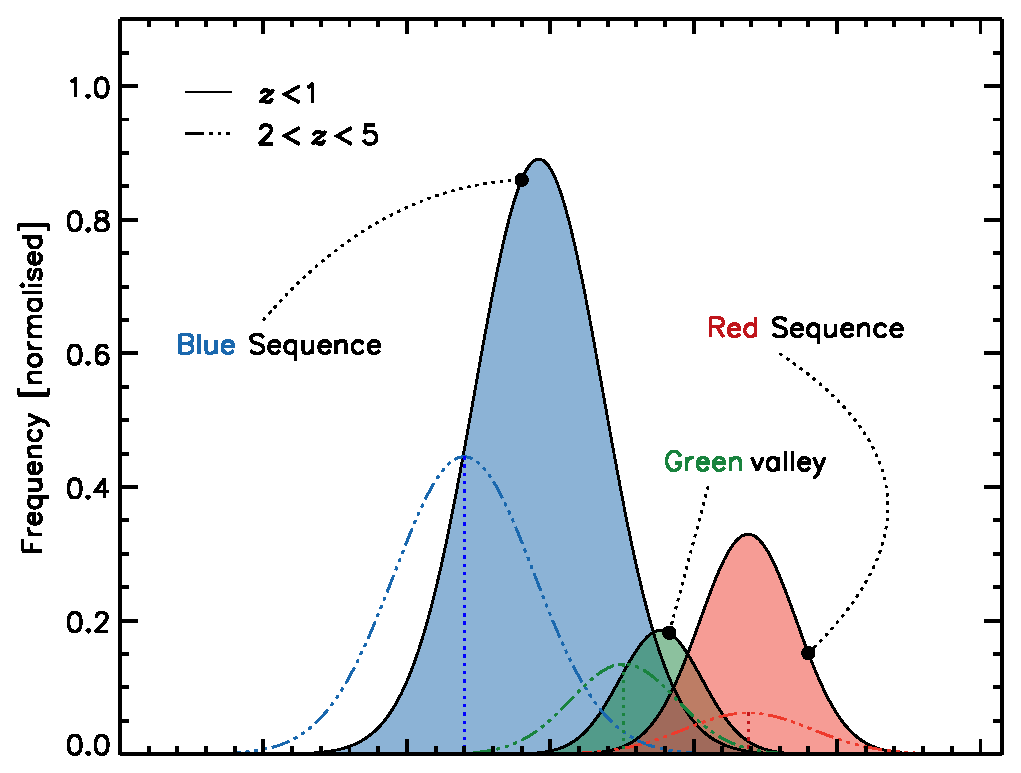
\includegraphics[width=\columnwidth]{nir_colour_template}\\
    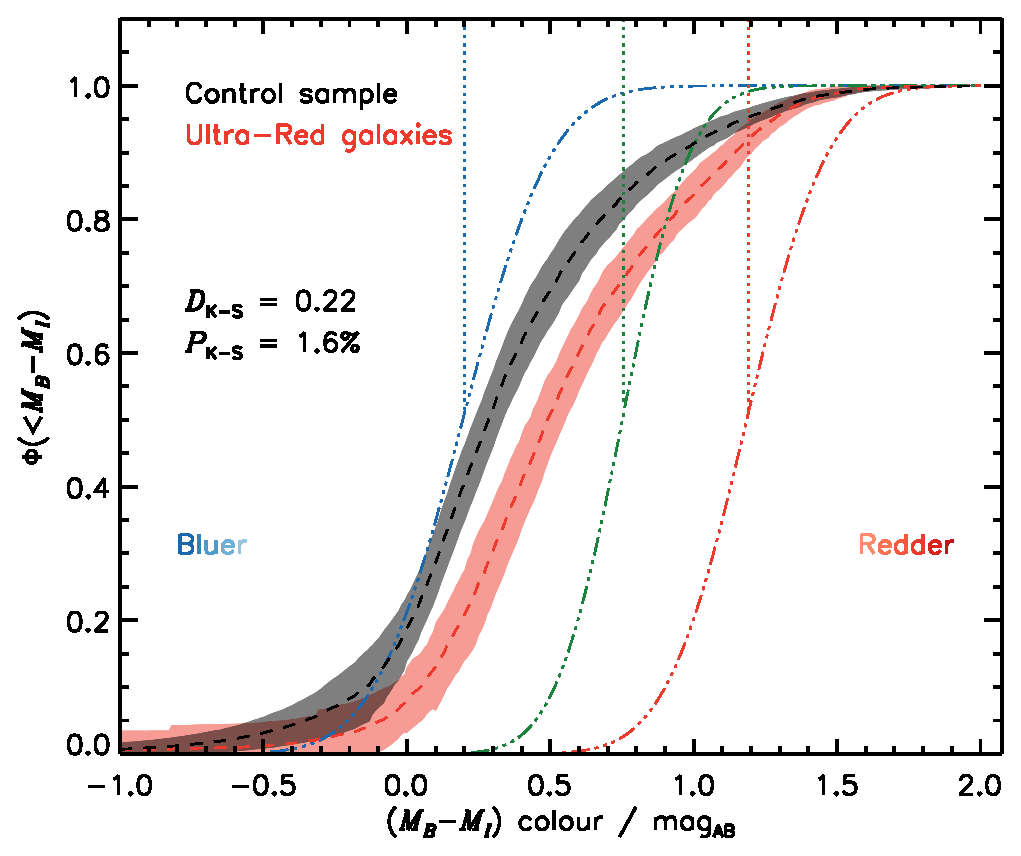
\includegraphics[width=\columnwidth]{nir_colour}
    \caption{%
    \textbf{Top:} empirically derived Gaussian distributions representing the red/blue sequences and so-called `green valley' at $z<1$ (solid lines) and $z\approx2\text{--}5$ (dashed lines).
    The distributions for the blue sequence and green valley are shifted to relatively bluer colours at $z\approx2\text{--}5$ compared to $z<1$ -- reflecting the prevalence of a younger stellar at these distant epochs.
    The peaks of these distributions at $z\approx2\text{--}5$ are indicated by dotted lines as an aid to the bottom panel of this figure.
    \textbf{Bottom:} CDF of the $(M_B - M_I)$ colour for LBGs detected within $\reff{}\approx5\arcmin$ of an \urg{} (red) or a random control position (black).
    LBGs from both samples have been weighted by their respective association probabilities using equation~(\ref{eq:vlos_assoc}).
    The CDFs for \urgs{} and the control sample diverge around $(M_B - M_I)=0.0\text{--}1.0$, which suggests that there is a larger number of red-sequence LBGs in the vicinity of \urgs{} than compared}
    \label{fig:nir_colour}
\end{figure}

\subsubsection[Dusty Surrounding NIR/Optical Galaxies]{Could the Surrounding NIR/Optical Galaxies Just be Dusty?}
\label{sec:av_extinct}

Although tentative evidence of the accelerated emergence of a red sequence around ultra-red galaxies has been presented in the previous section, we now analyse whether this same result could be achieved if the surrounding NIR/optical galaxies were simply dustier in composition, rather than `dead' in nature.

As the process of star formation increases the dust content in the ISM of star-bursting galaxies experiencing enhanced star formation, it is very plausible that the excess of red galaxies seen residing around ultra-red galaxies is due to a dustier population.
Such a scenario could hint at the presence of some large-scale mechanism capable of simultaneously enhancing the star formation across multiple galaxies within a dense environment \citepalias[see][]{lewis17}.

The variation of extinction with passband is usually defined using the $R_V$ parameter that takes into account the ratio of $V\text{-}$ and $B\text{-}$band extinction, or $A_V$ and $A_B$, respectively, as follows:
\begin{equation}
    R_V\equiv\frac{A_V}{A_B}-1,
\end{equation}

For the Milky Way or a starburst-like galaxy, $R_V$ typically ranges from $3.1\text{--}3.2$.
The magnitudes of extinction experienced by the $B\text{-}$ and $I$-bands assuming a value of $R_V=3.1$ are listed in Table~\ref{tab:av_extinct}.
Hence, the ($M_B-M_I$)-colour extinction (or $A_B - A_I$) can be defined as a function of $V$-band extinction as follows:
\begin{equation}
    \label{eq:av_extinct}
    A_B - A_I = (1.321-0.594)A_V \approx 0.7A_V,
\end{equation}
\noindent or equivalently, the $(M_B-M_I)$ colour is reddened by $\approx70\%$ of the $V\text{-}$band obscuration experienced by a given galaxy.

\begin{table} 
    \centering
    \caption[Magnitude variation with $V$-band extinction]{Magnitudes of extinction for the $B\text{-}$ and $I\text{-}$band photometry assuming the $R_V = 3.1$ extinction laws of \citet{cardelli89} and \citet{odonnell94}. \textbf{Note.} These data were obtained from \href{http://iopscience.iop.org/article/10.1086/305772/fulltext/tb6.gif}{Table~6} in \citet{schlegel98}.}
    \label{tab:av_extinct}
    \begin{tabular}{l c c c}
        \hline
        Facility & Filter & 1/$\lambda_{\text{eff}}$ & $A_{\lambda_{\text{eff}}}/A_V$ \\
         &  & $\micron{}^{-1}$ & \\
        \hline
        Subaru Suprime-Cam & $B$ & 2.3 & 1.3 \\
        Subaru Suprime-Cam & $I$ & 1.2 & 0.6 \\
        \hline
    \end{tabular}
\end{table}

In Fig.~\ref{fig:av_extinct}, we show the effect of increasing the $A_V$ extinction on the $(M_B-M_I)$ colour for the control sample by $A_V=(0\text{--}1)\,\magab{}$.
Clearly evident is that $A_V=1\,\magab{}$ of extinction shifts the control sample
to a redder $(M_B-M_I)$ colour (by $\approx0.5\,\magab{}$) than compared to the \urgs{}.

\begin{figure}
    \centering
    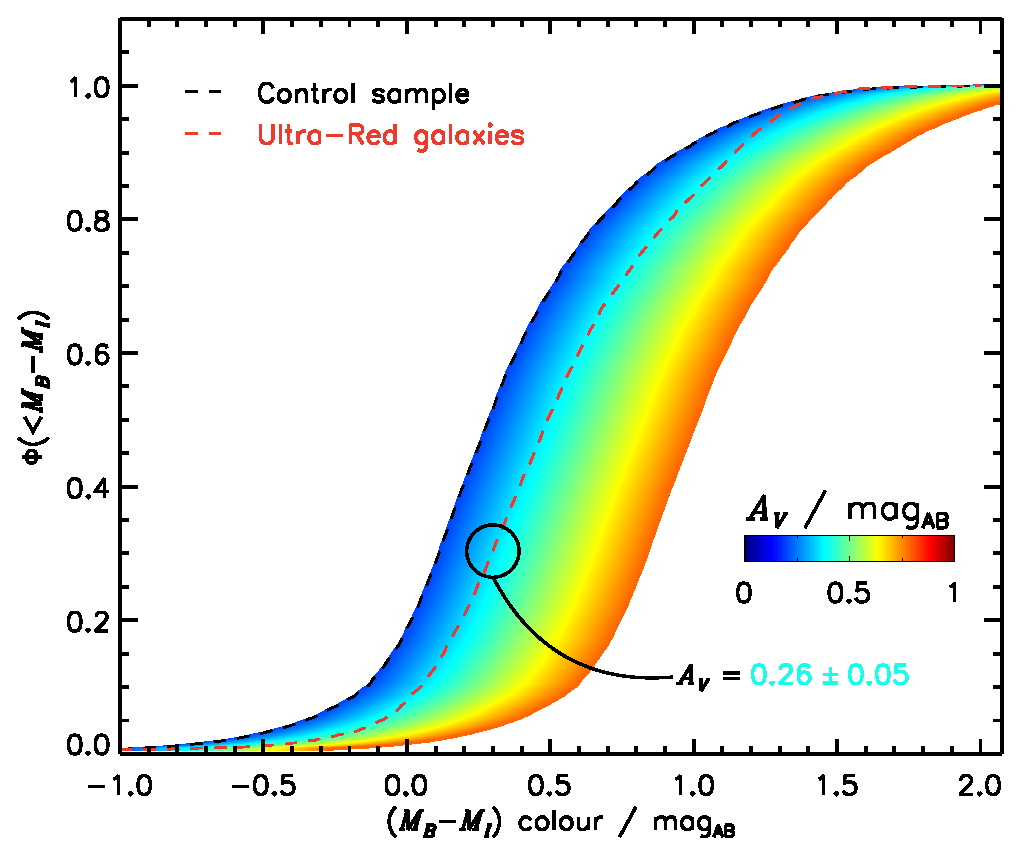
\includegraphics[width=\columnwidth]{av_extinct.eps}
    \caption[$(M_B-M_I)$ colour change with $V$-band extinction]{%\textbf{Main:}
    CDFs of the $(M_B-M_I)$ colour for the control sample and the \urgs{} as shown in Fig.~\ref{fig:nir_colour}.
    We adjust the $(M_B-M_I)$ colours of the control sample to account for varying amounts of $V$-band extinction up to $A_V=1\,\magab{}$ shown by the shaded region.
    Indicated by a black circle is the best-fit value of the extinction corrected CDF of the $(M_B-M_I)$ colour for the control sample to that of the \urgs{}.
    This best-fit, least-squares value suggests that the control sample could be mapped onto the \urg{} sample if they were to experience a very moderate dust reddening of $A_V\sim0.3\,\magab{}$.
    }
    \label{fig:av_extinct}
\end{figure}

Performing a least-squares fit to the $A_V$-corrected, $(M_B-M_I)$ colour of the control sample against the $(M_B-M_I)$ colour of the \urgs{} yields a value of $A_V\sim(0.26\pm0.05)\,\magab{}$.
Thus, the control sample \emph{could} be mapped onto the \urg{} sample if it was to 
experience a very moderate dust reddening of $A_V\sim0.3\,\magab{}$.

Thus, it is very plausible that the optical/NIR galaxies surrounding \urgs{} are experiencing enhanced star formation that is slightly increasing the amount of dust within their ISM.

\subsection{Over-Densities of LBGs}

We computed the optical/NIR over-density parameters around the \urgs{} by comparing the number of massive $\mstars{}>10^{10}\text{-}\msol{}$ galaxies residing in their $5\text{-}\text{arcmin}$ environments to that expected from the field.
Throughout this calculation, we took into account the varying instrumental noise and edge effects by `conserving' the number of pixels within each $5\text{-}\text{arcmin}$ aperture around the positions of \urgs{} and their respective control samples.

\begin{figure*}
    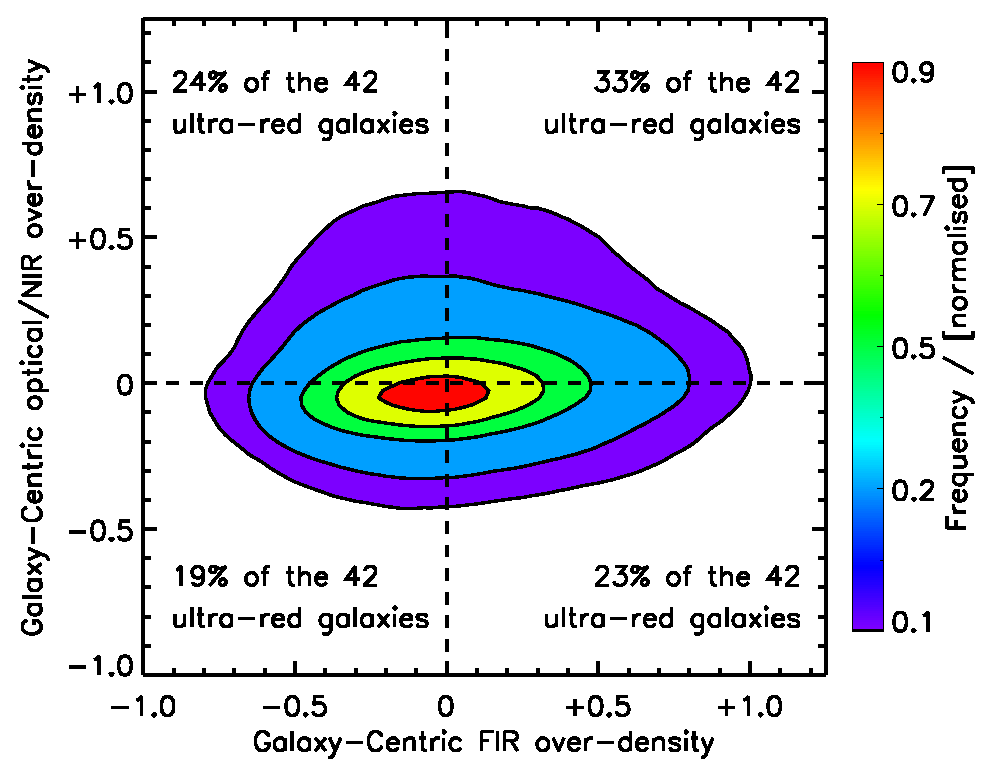
\includegraphics[width=1.25\columnwidth]{delta_nir_vs_fir}
    \caption{Optical/NIR versus FIR over-densities for the $42$ \urgs{} with optical/NIR data.
    \textbf{Note.\ } The comparatively low over-density parameter values reported here are due to the large apertures over which they are measured that effectively dilutes the signal from all but the largest over-densities.}
    \label{fig:delta_nir_vs_fir}
\end{figure*}


In Fig.~\ref{fig:delta_nir_vs_fir}, we show how these optical/NIR over-densities vary as a function of the FIR over-densities computed previously.
Thus, it would appear that not all over-densities of DSFGs equate to over-densities of LBGs, at least not \emph{strongly} since there does appear to be a \emph{slight} tilt in the contours, which may suggest that they may correlate weakly.
However, only $\sim60\%$ of the $32$ \urgs{} with available optical/NIR data reside in over-dense regions of the Universe, and of these, only $\sim60\%$ are over-dense in LBGs.
Or put another way, only a third of \urgs{} appear to be over-dense in both DSFGs \emph{and} LBGs.
Overall though, $\sim80\%$ of \urgs{} signpost regions that are either over-dense in DSFGs, or LBGs or both.

\section{Conclusion}

In this paper, we have presented a multi-wavelength analysis of $64$ \urgs{} -- selected via their ultra-red probabilities -- within the S2CLS and S2COSMOS imaging surveys.

We found that just over half of these \urgs{} reside in over-dense regions of DSFGs.
In terms of global FIR over-density peaks, it appears that \urgs{} play a central ($<$ a few megaparsec) role in medium-value global over-density peaks.
By weighting each DSFG by its probability of being associated to the central \urg{}, we found that the average total dust masses surrounding these \urgs{} was $\sim2\times10^{9}\,\msol{}$ (having been corrected for the `missing' DSFGs within their vicinities).
These values are consistent with those reported in \citetalias{lewis17}.
However, we were still only able to associate $\approx1$ surrounding DSFG to its central \urg{} using this new association method, which perhaps suggests that this is the limit achievable with FIR-based photometric redshifts.

Using optical/NIR ground-based data (down to $5\text{-}\sigma_{K}$ depths of $\lesssim24\,\magab{}$) for $32$ \urgs{} within the COSMOS and UDS fields, we were able to associate an average of $\approx28$ LBGs to within $\lesssim5\arcmin{}$ of a given \urg{} -- a factor of $\sim30\times$ the number of DSFGs.
These associated LBGs showed a factor of $\approx5\times$ increase in stellar mass and a factor of $3\times$ increase in absolute ($M_{B}-M_{I}$) colour as their distance to the \urgs{} decreased over $\approx500\,\kiloparsec{}$ (or $\approx2\arcmin{}$) scales.
This suggests that the red sequence has already emerged, or is beginning to emerge, around these \urgs{} at $z\sim3$.
In particular, there appears to be a higher fraction of green-valley galaxies around \urgs{} than compared to the field, supporting the concept that, on average, the red sequence is emerging at a faster rate around \urgs{}.
With an average total stellar mass contribution from the LBGs of $4.7\times10^{11}\,\msol{}$, and assuming that the \urgs{} convert all of their molecular gas into stars, these candidate, high-redshift proto-clusters have the potential to form systems with stellar masses of at least $\mstars{}\sim10^{12}\,\msol{}$ by $z\sim0$.

Thus, we have shown that there is a sizeable contribution from LBGs to these high-redshift systems signposted by \urgs{}.
Although these systems have average optical/NIR/FIR properties that are consistent with their evolution into present-day galaxy clusters with DM halos of mass $\mhalo{}\sim10^{14}\text{--}10^{15}\,\msol{}$, we are still likely missing a sizeable contribution from LBGs that my association probability has failed to associate.
Therefore, the results presented here should be regarded as firm lower limits on the optical/NIR/FIR properties of the environments around \urgs{}, which can now only be improved upon when spectroscopic data increases the accuracy of the redshift estimates.

\section*{Acknowledgements}

AJRL and RJI acknowledge support from the European Research Council (ERC) in the form of Advanced Grant, 321302, \textsc{cosmicism}.
%
This research has made use of data from \hermes{} project
(\url{http://hermes.sussex.ac.uk/}). \hermes{} is a \herschel{} Key
Programme utilizing Guaranteed Time from the SPIRE instrument team, ESAC
scientists and a mission scientist.
%
The JCMT is operated by the East Asian Observatory on behalf of The National Astronomical Observatory of Japan, Academia Sinica Institute of Astronomy and Astrophysics, the Korea Astronomy and Space Science Institute, the National Astronomical Observatories of China and the Chinese Academy of Sciences (Grant No.~XDB09000000), with additional funding support from STFC and participating universities in the UK and Canada; Program ID MJLSC0.

\bibliographystyle{mnras}
\bibliography{lewis-mnras-2018.bib}

\appendix

\section{Ultra-Red Over-Density and Herschel SPIRE Cut-Outs}
\label{app:cut_outs}

In this Appendix, we present the over-density and \herschel{} SPIRE cut-outs for the remaining \urgs{} with $\pur{}>60\%$.

\begin{figure*}
    \centering
    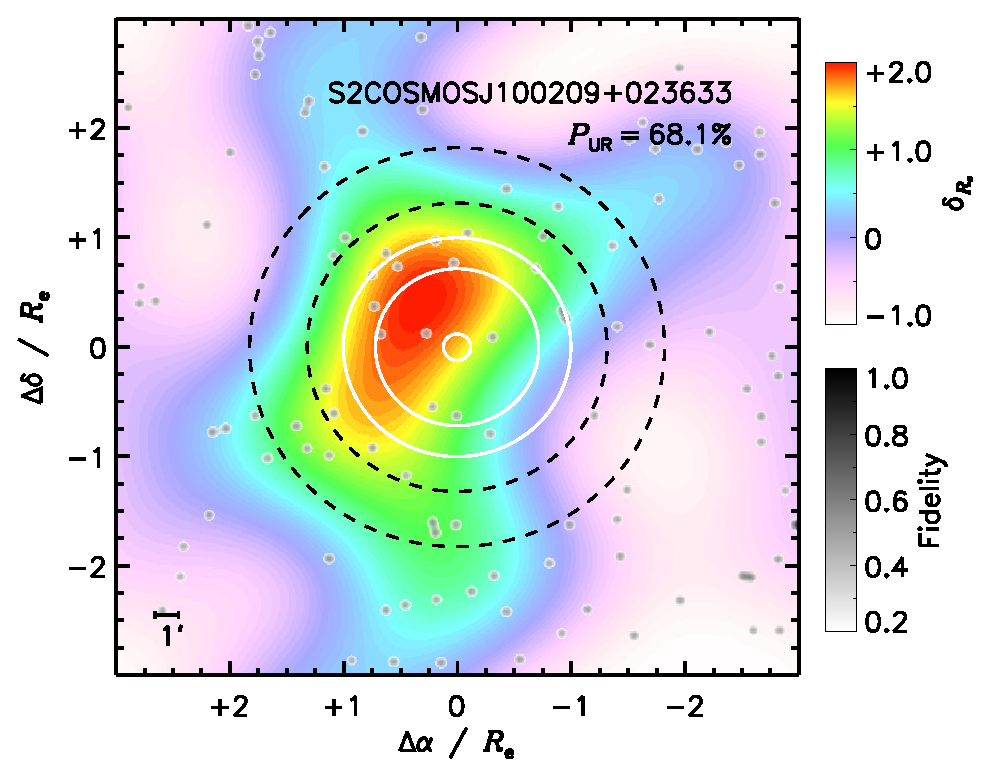
\includegraphics[width=0.5\textwidth]{S2COSMOSJ100209+023633-overdensity}
    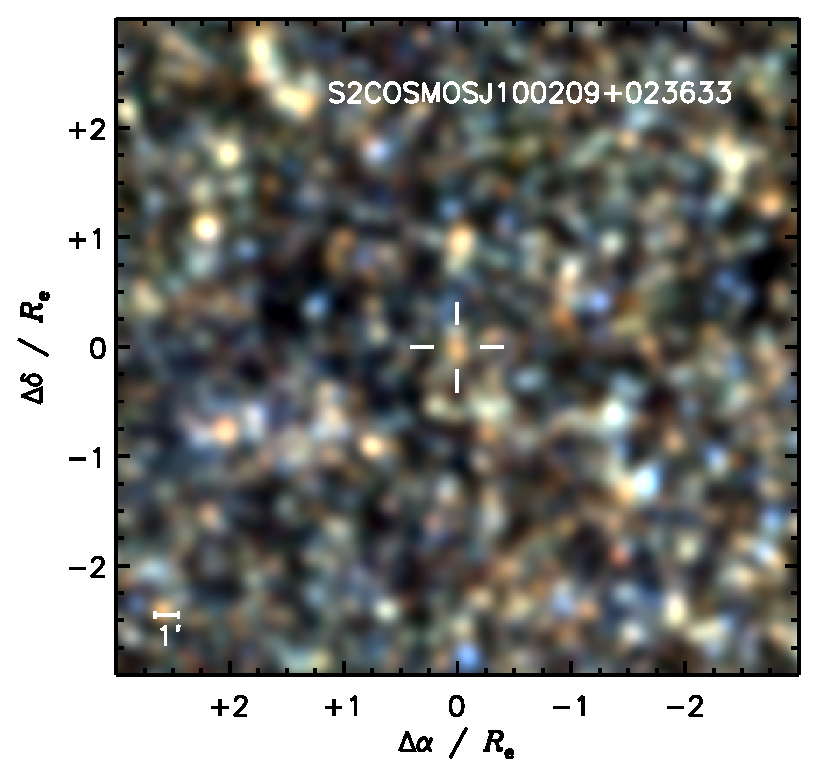
\includegraphics[width=0.41\textwidth]{S2COSMOSJ100209+023633-spire-rgb}\\\vspace{1em}
    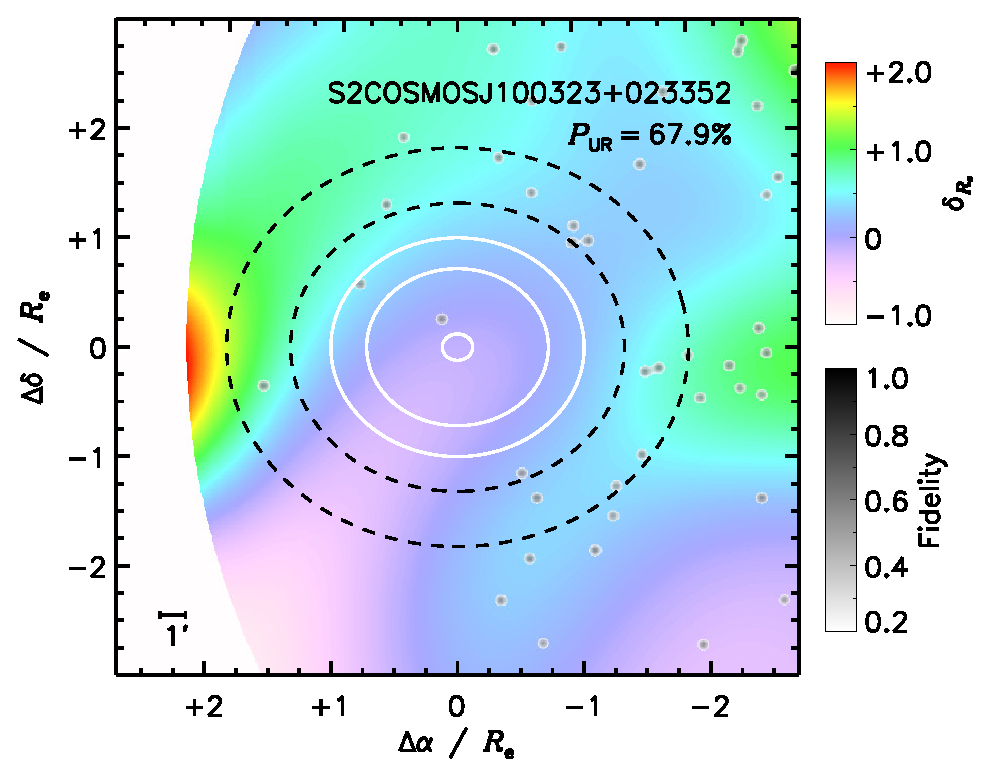
\includegraphics[width=0.5\textwidth]{S2COSMOSJ100323+023352-overdensity}
    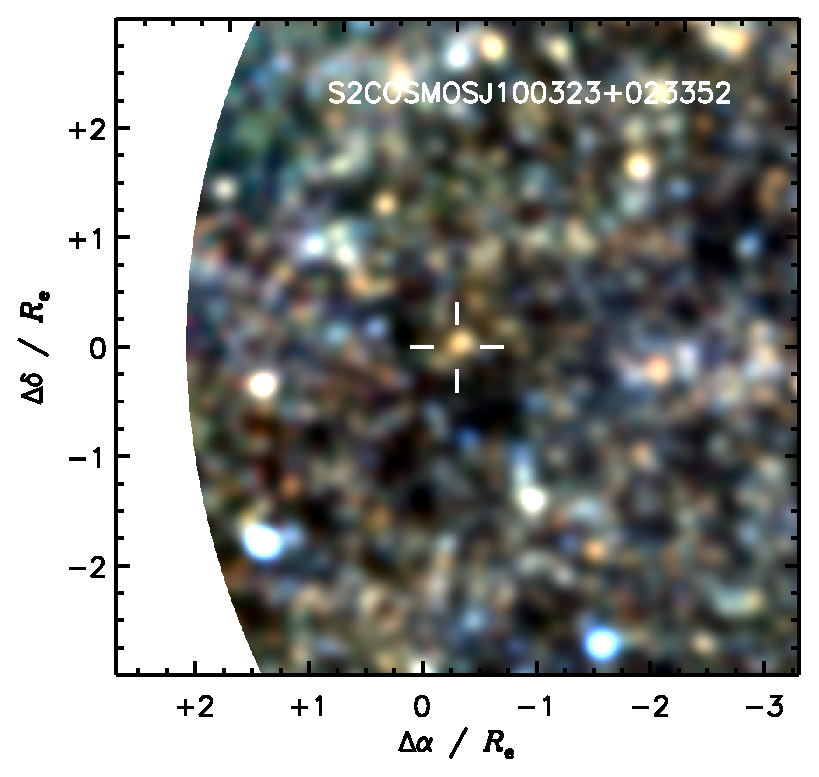
\includegraphics[width=0.41\textwidth]{S2COSMOSJ100323+023352-spire-rgb}\\\vspace{1em}
    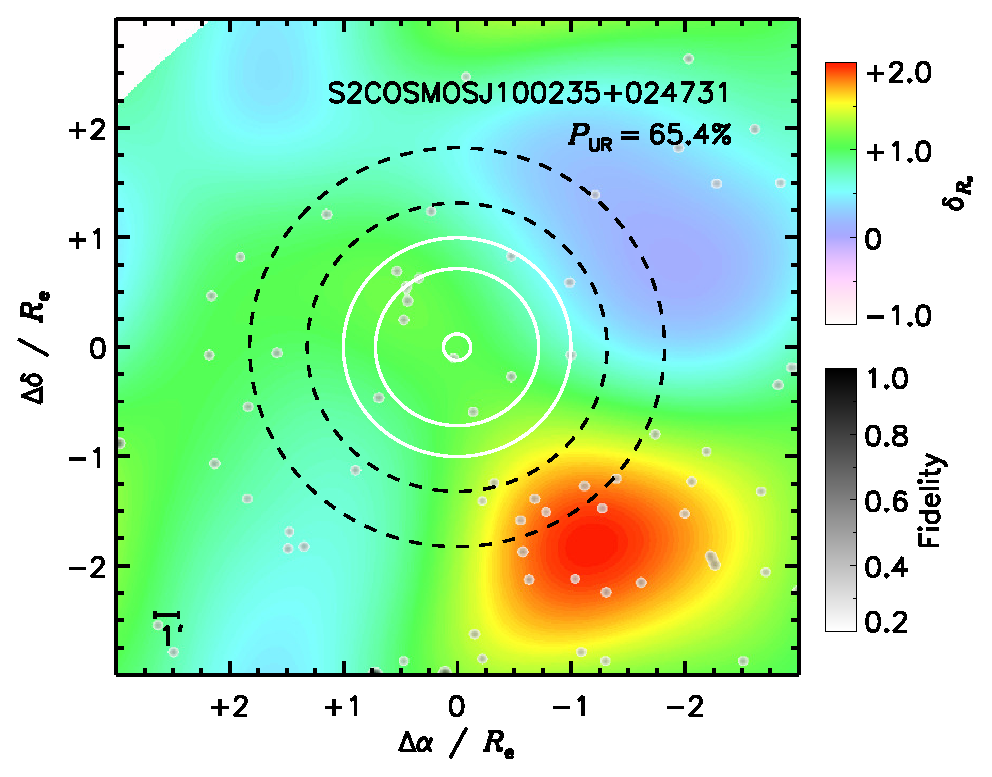
\includegraphics[width=0.5\textwidth]{S2COSMOSJ100235+024731-overdensity}
    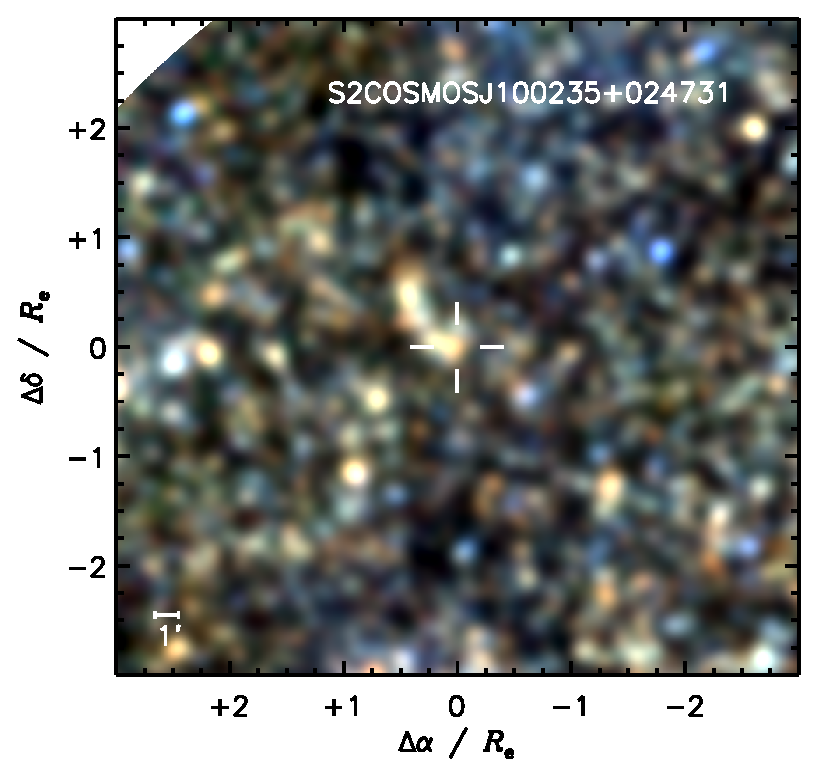
\includegraphics[width=0.41\textwidth]{S2COSMOSJ100235+024731-spire-rgb}
    \caption{Continuation of Fig.~\ref{fig:s2cls_cut_outs} \ldots}
    \label{fig:this_figure}
\end{figure*}

\addtocounter{figure}{-1}
\begin{figure*}
    \centering
    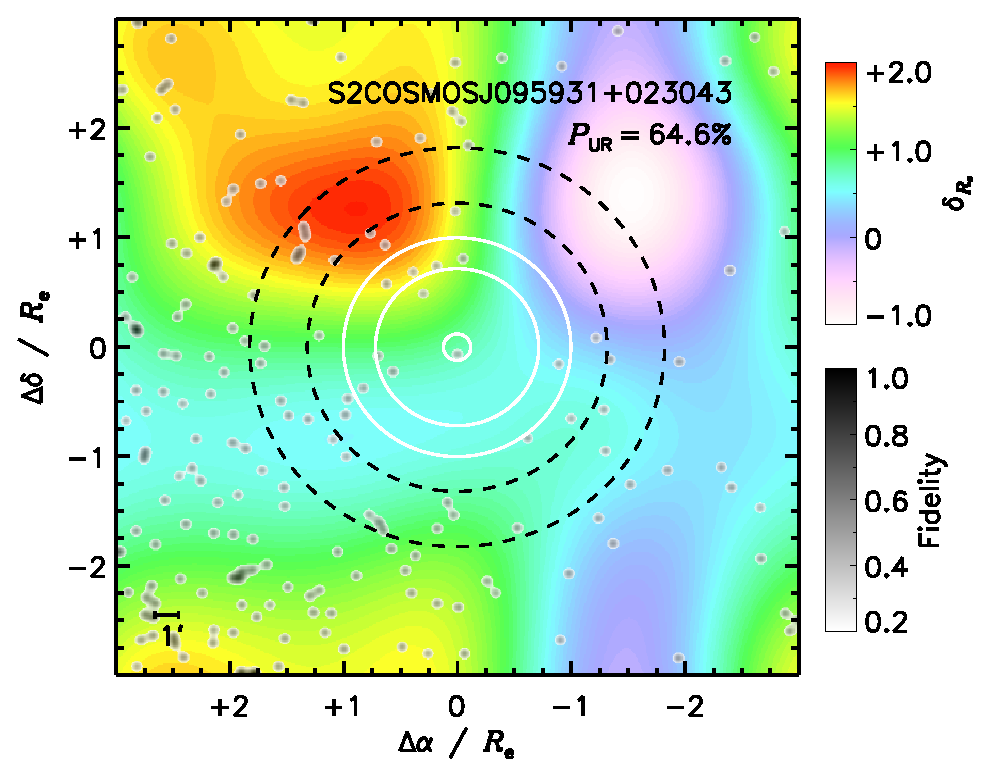
\includegraphics[width=0.5\textwidth]{S2COSMOSJ095931+023043-overdensity}
    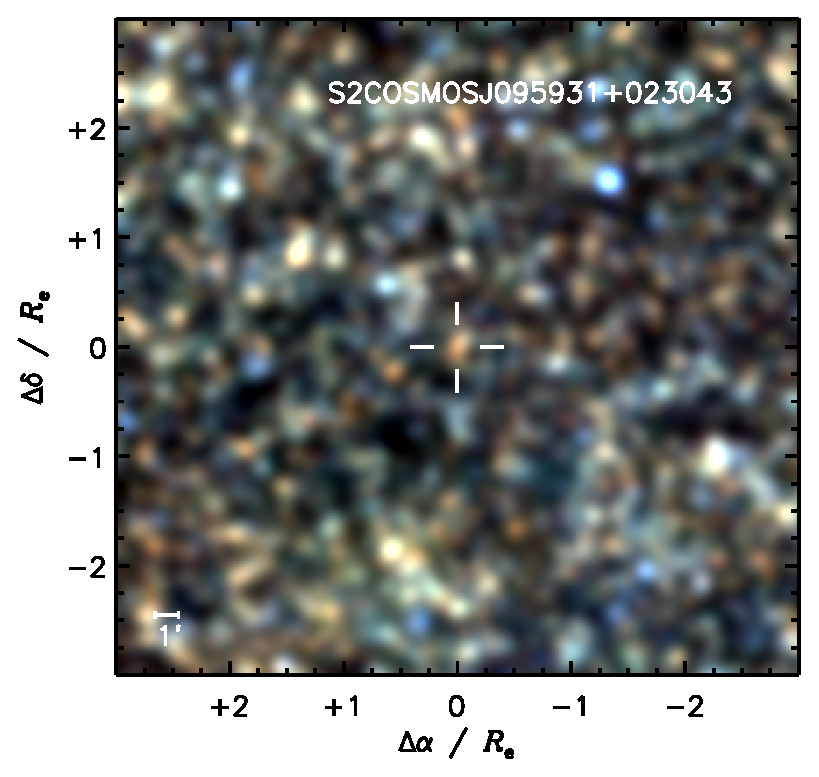
\includegraphics[width=0.41\textwidth]{S2COSMOSJ095931+023043-spire-rgb}\\\vspace{1em}
    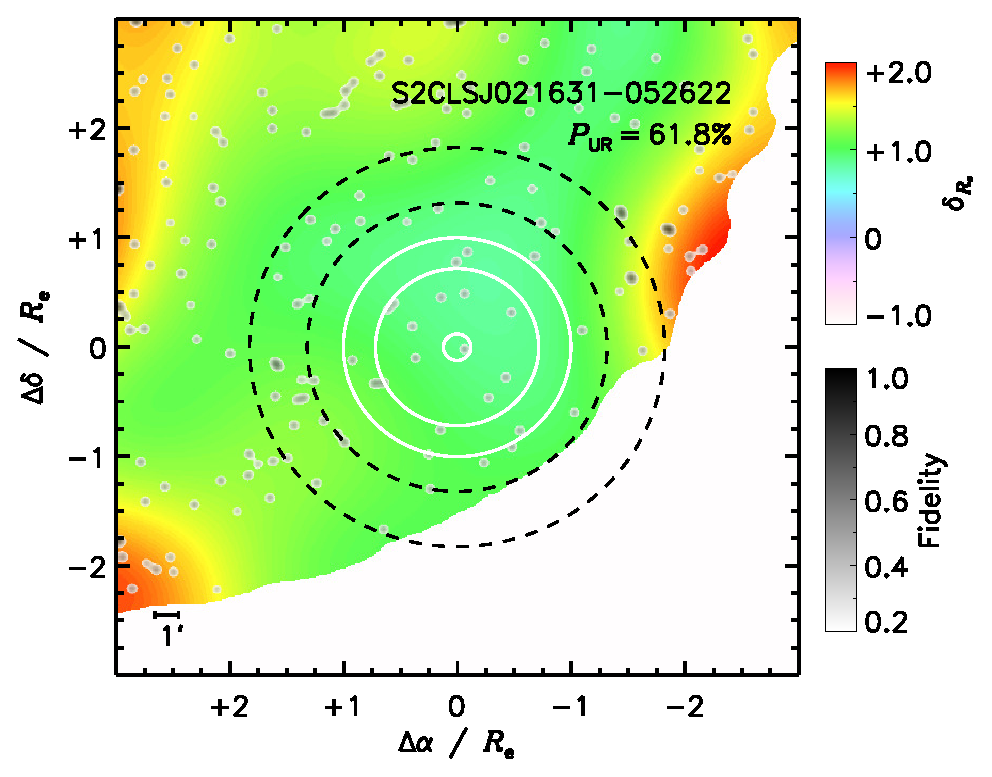
\includegraphics[width=0.5\textwidth]{S2CLSJ021631-052622-overdensity}
    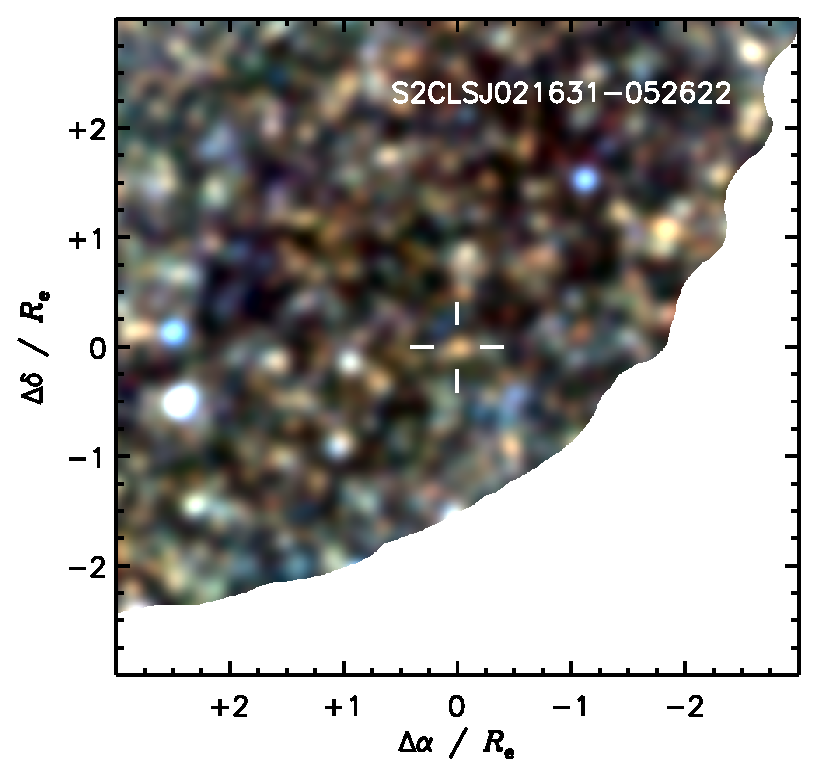
\includegraphics[width=0.41\textwidth]{S2CLSJ021631-052622-spire-rgb}\\\vspace{1em}
    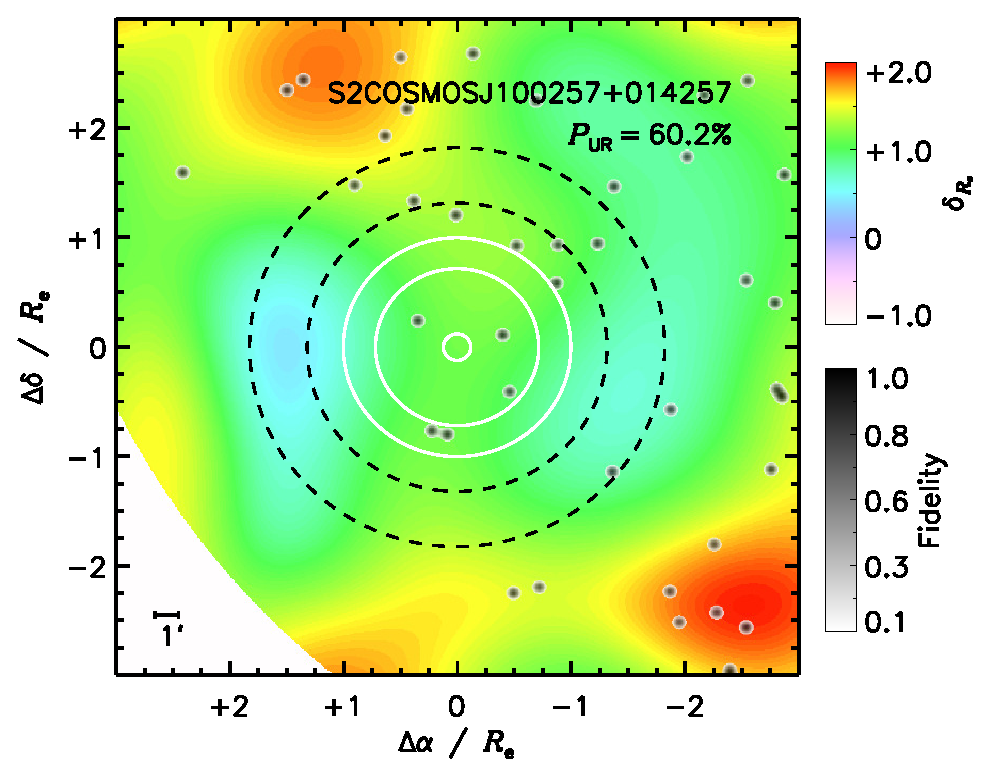
\includegraphics[width=0.5\textwidth]{S2COSMOSJ100257+014257-overdensity}
    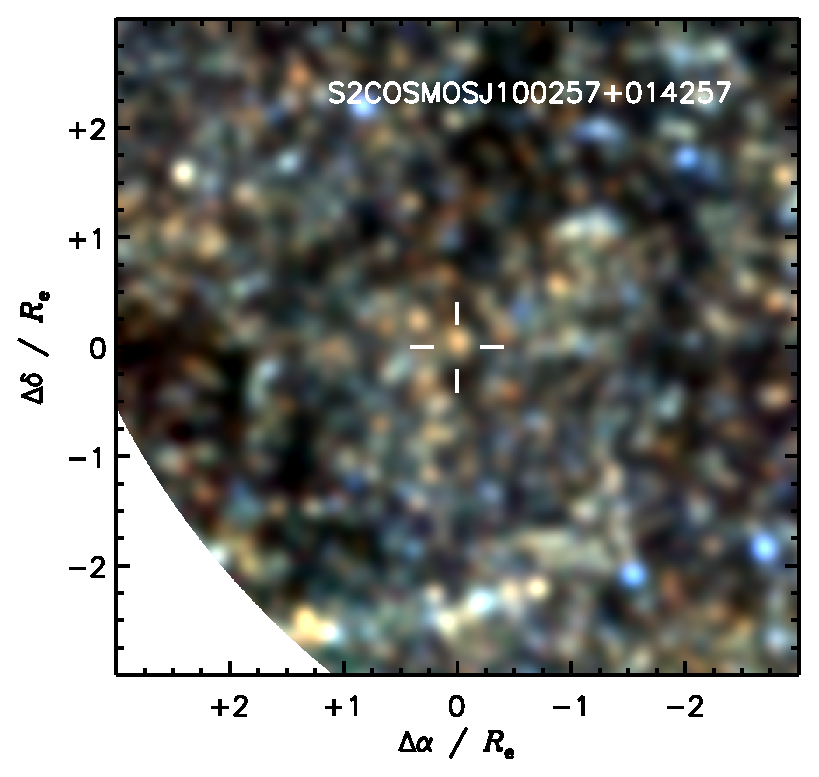
\includegraphics[width=0.41\textwidth]{S2COSMOSJ100257+014257-spire-rgb}
    \caption{Continuation of Fig.~\ref{fig:s2cls_cut_outs} \ldots}
\end{figure*}


% Don't change these lines
\bsp	% typesetting comment
\label{lastpage}
\end{document}
